\section{Casi d'uso}

		% LEGGE DI MAXELWEB
		% (NICE > OK)
		% [log_13-01-2020] Lasciate ogni speranza a voi che entrate. In questa terra proibita in data Lun 13 gennaio 2019 si è consumato il caos che ha portato alla creazione di 136 casi d'uso. Non sappiamo ancora se saremo salvi dallo sciagurato esito del RR. L'inverno sta arrivando. Il freddo è tra noi. La pazzia si dilata dalle nostre ossa. Scappate finche siete in tempo. Scappate!

		\subsection{Contesto riassuntivo per l'accesso alla web app}

		\begin{figure}[H]
			\centering
			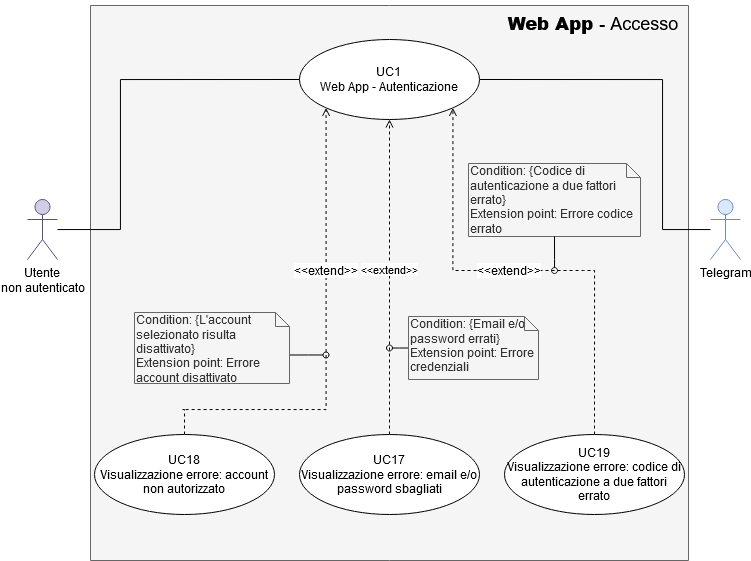
\includegraphics[scale=0.6]{res/images/webapp-accesso}
			\caption{Diagramma riassuntivo che illustra la parte di autenticazione alla web app.}
		\end{figure}

		% =================
		% UC 1 [NICE]

			\subsection{UC1 - Web App - Autenticazione}
		
	\begin{figure}[H]
		\centering
		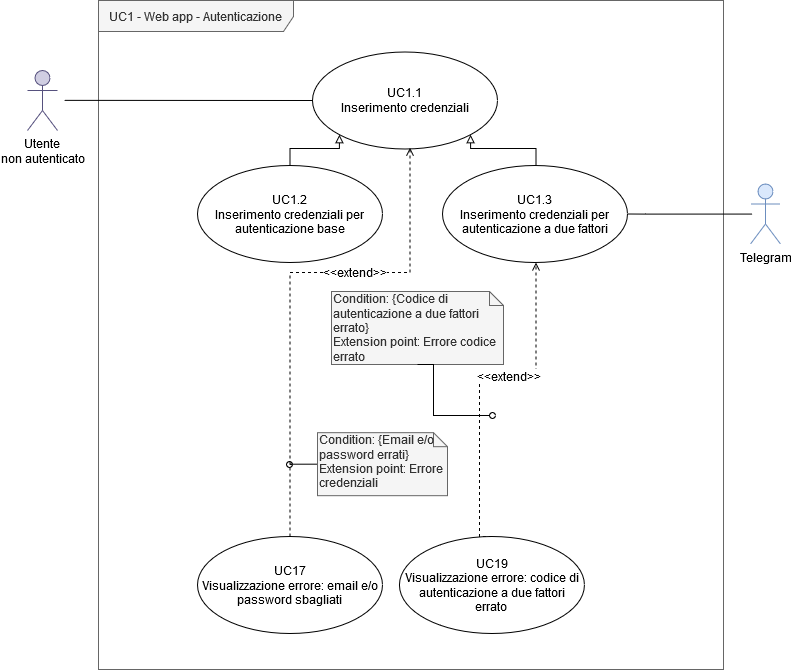
\includegraphics[scale=0.60]{res/images/uc1}
		\caption{Diagramma che riassume il processo di autenticazione nella web app.}
	\end{figure}
		
	\begin{itemize}
		\item \textbf{Attori Primari}: Utente non autenticato.
		\item \textbf{Attori Secondari}: \glock{Telegram}.
		\item \textbf{Descrizione}: L'utente vuole autenticarsi nella web app, per poter accedere alle funzionalità del sito.
		\item \textbf{Precondizione}: L'utente non è autenticato nella web app.
		\item \textbf{Postcondizione}: L'utente effettua l'autenticazione nella web app.
		\item \textbf{Scenario Principale}:
		\begin{enumerate}
			\item L'utente inserisce le proprie credenziali (UC 1.1);
			\item Viene eseguito il controllo delle credenziali inserite (UC 1.4).
		\end{enumerate}
	\end{itemize}
	

		\subsubsection{UC 1.1 - Inserimento credenziali}

		\begin{itemize}
			\item \textbf{Attori Primari}: Utente non autenticato.
			\item \textbf{Descrizione}: L'utente vuole autenticarsi nella web app e deve inserire alcuni campi obbligatori per procedere.
			\item \textbf{Precondizione}: L'utente non è autenticato nella web app.
			\item \textbf{Postcondizione}: L'utente ha inserito le credenziali richieste.
			\item \textbf{Scenario Principale}:
			\begin{enumerate}
				\item L'utente inserisce le credenziali per l'autenticazione base (UC 1.2);
				\item L'utente inserisce le credenziali per l'autenticazione a due fattori (UC 1.3);
			\end{enumerate}
			\item \textbf{Inclusioni}:
				\begin{itemize}
					\item Controllo credenziali (UC 1.4).
				\end{itemize}
			\item \textbf{Estensioni}:
				\begin{itemize}
					\item Visualizzazione errore: email e/o una password errati (UC 17).
				\end{itemize}
		\end{itemize}

		\subsubsection{UC 1.2 - Inserimento credenziali per autenticazione base}

		\begin{figure}[H]
			\centering
			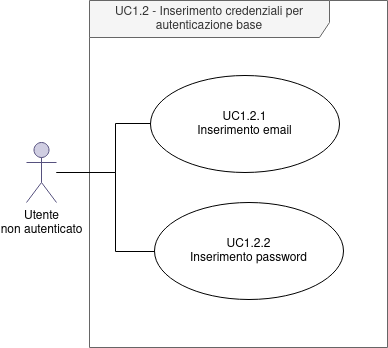
\includegraphics[scale=0.675]{res/images/uc1.2}
			\caption{Diagramma che descrive l'inserimento delle credenziali per l'autenticazione base.}
		\end{figure}

		\begin{itemize}
			\item \textbf{Attori Primari}: Utente non autenticato.
			\item \textbf{Descrizione}: L'utente vuole autenticarsi nella web app ed inserisce i campi obbligatori per l'autenticazione base.
			\item \textbf{Precondizione}: L'utente non è autenticato nella web app.
			\item \textbf{Postcondizione}: L'utente ha inserito le credenziali richieste.
			\item \textbf{Scenario Principale}:
			\begin{enumerate}
				\item L'utente inserisce la email (UC 1.2.1);
				\item L'utente inserisce la password (UC 1.2.2).
			\end{enumerate}	
		\end{itemize}

			\paragraph{UC 1.2.1 - Inserimento email}
			\begin{itemize}
				\item \textbf{Attori Primari}: Utente non autenticato.
				\item \textbf{Descrizione}: L'utente vuole autenticarsi nella web app e inserisce uno dei campi obbligatori per l'autenticazione base.
				\item \textbf{Precondizione}: L'utente non è autenticato nella web app.
				\item \textbf{Postcondizione}: L'utente ha inserito la credenziale richiesta.
				\item \textbf{Scenario Principale}:
				\begin{enumerate}
					\item L'utente compila il campo email.
				\end{enumerate}	
			\end{itemize}

			\paragraph{UC 1.2.2 - Inserimento password}
			\begin{itemize}
				\item \textbf{Attori Primari}: Utente non autenticato.
				\item \textbf{Descrizione}: L'utente vuole autenticarsi nella web app e inserisce uno dei campi obbligatori per l'autenticazione base.
				\item \textbf{Precondizione}: L'utente non è autenticato nella web app.
				\item \textbf{Postcondizione}: L'utente ha inserito la credenziale richiesta.
				\item \textbf{Scenario Principale}:
				\begin{enumerate}
					\item L'utente compila il campo password.
				\end{enumerate}	
			\end{itemize}

		\subsubsection{UC 1.3 - Inserimento credenziali per autenticazione a due fattori}

		\begin{figure}[H]
			\centering
			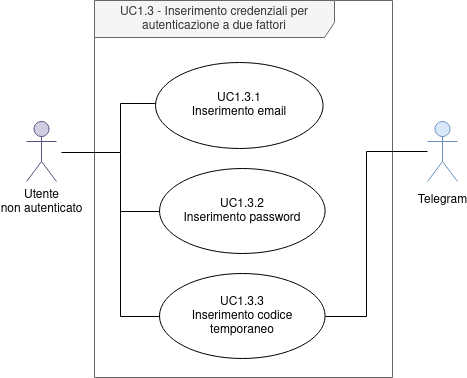
\includegraphics[scale=0.675]{res/images/uc1.3}
			\caption{Diagramma che descrive l'inserimento delle credenziali per l'autenticazione a due fattori.}
		\end{figure}

		\begin{itemize}
			\item \textbf{Attori Primari}: Utente non autenticato.
			\item \textbf{Attori Secondari}: \glock{Telegram}.
			\item \textbf{Descrizione}: L'utente vuole autenticarsi nella web app ed inserisce i campi obbligatori per l'autenticazione a due fattori.
			\item \textbf{Precondizione}: L'utente non è autenticato nella web app.
			\item \textbf{Postcondizione}: L'utente ha inserito le credenziali richieste.
			\item \textbf{Scenario Principale}:
				\begin{enumerate}
					\item L'utente inserisce la email (UC 1.3.1);
					\item L'utente inserisce la password (UC 1.3.2);
					\item L'utente inserisce un codice temporaneo ricevuto tramite \glock{Telegram} (UC 1.3.3).
				\end{enumerate}
			\item \textbf{Estensioni}:
				\begin{itemize}
					\item Visualizzazione errore: codice di autenticazione a due fattori errato (UC 19).
				\end{itemize}	
		\end{itemize}

			\paragraph{UC 1.3.1 - Inserimento email}
			\begin{itemize}
				\item \textbf{Attori Primari}: Utente non autenticato.
				\item \textbf{Descrizione}: L'utente vuole autenticarsi nella web app e inserisce uno dei campi obbligatori per l'autenticazione a due fattori.
				\item \textbf{Precondizione}: L'utente non è autenticato nella web app.
				\item \textbf{Postcondizione}: L'utente ha inserito la credenziale richiesta.
				\item \textbf{Scenario Principale}:
				\begin{enumerate}
					\item L'utente compila il campo email.
				\end{enumerate}	
			\end{itemize}

			\paragraph{UC 1.3.2 - Inserimento password}
			\begin{itemize}
				\item \textbf{Attori Primari}: Utente non autenticato.
				\item \textbf{Descrizione}: L'utente vuole autenticarsi nella web app e inserisce uno dei campi obbligatori per l'autenticazione a due fattori.
				\item \textbf{Precondizione}: L'utente non è autenticato nella web app.
				\item \textbf{Postcondizione}: L'utente ha inserito la credenziale richiesta.
				\item \textbf{Scenario Principale}:
				\begin{enumerate}
					\item L'utente compila il campo password.
				\end{enumerate}	
			\end{itemize}

			\paragraph{UC 1.3.3 - Inserimento codice temporaneo}
			\begin{itemize}
				\item \textbf{Attori Primari}: Utente non autenticato.
				\item \textbf{Attori Secondari}: \glock{Telegram}.
				\item \textbf{Descrizione}: L'utente vuole autenticarsi nella web app e inserisce uno dei campi obbligatori per l'autenticazione a due fattori.
				\item \textbf{Precondizione}: L'utente non è autenticato nella web app.
				\item \textbf{Postcondizione}: L'utente ha inserito la credenziale richiesta.
				\item \textbf{Scenario Principale}:
				\begin{enumerate}
					\item L'utente riceve una notifica tramite \glock{Telegram} con un codice temporaneo;
					\item L'utente compila il campo codice temporaneo.
				\end{enumerate}	
			\end{itemize}


		


		\subsection{Contesto riassuntivo per le interazioni nella web app}

		\begin{figure}[H]
			\centering
			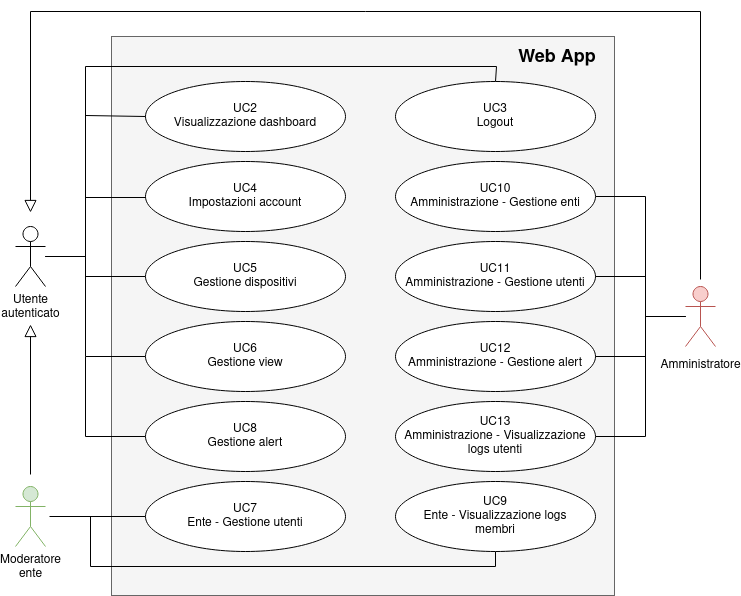
\includegraphics[scale=0.6]{res/images/webapp}
			\caption{Diagramma riassuntivo che illustra le interazioni principali all'interno della web app.}
		\end{figure}


		% =================
		% UC 2 [NICE]

		\subsection{UC 2 - Visualizzazione Dashboard}
		
		\begin{itemize}
			\item \textbf{Attori Primari}: Utente autenticato.
			\item \textbf{Descrizione}: L'utente ha eseguito l'autenticazione e vuole visualizzare una dashboard con all'interno le proprie informazioni account, alcune statistiche del sito e le informazioni di supporto tecnico.
			\item \textbf{Precondizione}: L'utente è autenticato nella web app.
			\item \textbf{Postcondizione}: L'utente visualizza la dashboard con le proprie informazioni.
			\item \textbf{Scenario Principale}:
			\begin{enumerate}
				\item Nella web app, l'utente può navigare per giungere alla visualizzazione della dashboard.
			\end{enumerate}	
		\end{itemize}

		% =================
		% UC 3 [NICE]

		\subsection{UC 3 - Logout}
		\begin{itemize}
			\item \textbf{Attori Primari}: Utente autenticato.
			\item \textbf{Descrizione}: L'utente vuole eseguire l'uscita dalla web app.
			\item \textbf{Precondizione}: L'utente risulta essere autenticato nella web app.
			\item \textbf{Postcondizione}: L'utente non è più autenticato nella web app.
			\item \textbf{Scenario Principale}:
			\begin{enumerate}
				\item L'utente effettua il logout;
				\item L'utente ritorna alla schermata di autenticazione per l'accesso alla web app.
			\end{enumerate}	
		\end{itemize}

		% =================
		% UC 4 - [NICE]

			\subsection{UC 4 - Impostazioni Account}
		
		\begin{figure}[H]
			\centering
			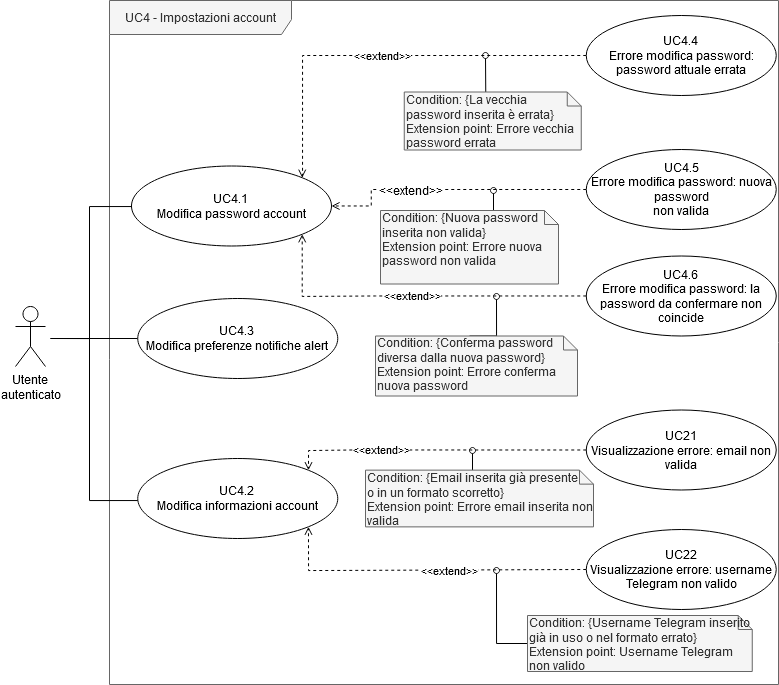
\includegraphics[scale=0.60]{res/images/uc4}
			\caption{Diagramma che riassume le interazioni con le impostazioni del proprio account.}
		\end{figure}
		
		\begin{itemize}
			\item \textbf{Attori Primari}: Utente autenticato.
			\item \textbf{Descrizione}: L'utente ha la possibilità di gestire le proprie impostazioni account, tra cui la modifica della password, le preferenze di notifica e le informazioni a lui associate.
			\item \textbf{Precondizione}: L'utente risulta autenticato all'interno della web app.
			\item \textbf{Postcondizione}: L'utente ha aggiornato le proprie impostazioni.
			\item \textbf{Scenario Principale}:
			\begin{enumerate}
				\item{L'utente naviga all'interno delle impostazioni del proprio account}
				\item{L'utente modifica le proprie impostazioni}
				\item{L'utente ha aggiornato le proprie impostazioni}
			\end{enumerate}	
		\end{itemize}
			

			\subsubsection{UC 4.1 - Modifica password account}
			\begin{itemize}
				\item \textbf{Attori Primari}: Utente autenticato.
				\item \textbf{Descrizione}: L'utente può cambiare la password associata al proprio account.
				\item \textbf{Precondizione}: L'utente naviga all'interno delle sue impostazioni.
				\item \textbf{Postcondizione}: L'utente ha cambiato la propria password.
				\item \textbf{Scenario Principale}:
				\begin{enumerate}
					\item L'utente deve inserire dei campi obbligatori per proseguire;
					\item L'utente inserisce il campo per la password attuale (4.1.1);
					\item L'utente inserisce il campo per la nuova password (4.1.2);
					\item L'utente inserisce il campo per la conferma della nuova password (4.1.3);
					\item L'utente ha cambiato la propria password.
				\end{enumerate}	
				\item \textbf{Estensioni}:
					\begin{itemize}
						\item Errore modifica password: password attuale errata (UC 4.4)
						\item Errore modifica password: nuova password non valida (UC 4.5)
						\item Errore modifica password: la password da confermare non coincide co la nuova password (UC 4.6)
					\end{itemize}
			\end{itemize}

				\paragraph{UC 4.1.1 - Inserimento password attuale}
				\begin{itemize}
					\item \textbf{Attori Primari}: Utente autenticato.
					\item \textbf{Descrizione}: Per proseguire nella modifica password, l'utente deve inserire la sua password attuale associata all'account. Il campo è obbligatorio.
					\item \textbf{Precondizione}: L'utente è all'interno delle sue impostazioni account.
					\item \textbf{Postcondizione}: L'utente ha compilato il campo richiesto.
					\item \textbf{Scenario Principale}:
					\begin{enumerate}
						\item L'utente compila il campo per la password attuale.
					\end{enumerate}
				\end{itemize}

				\paragraph{UC 4.1.2 - Inserimento nuova password}
				\begin{itemize}
					\item \textbf{Attori Primari}: Utente autenticato.
					\item \textbf{Descrizione}: Per proseguire nella modifica password, l'utente deve scegliere e inserire una nuova password. Il campo è obbligatorio.
					\item \textbf{Precondizione}: L'utente è all'interno delle sue impostazioni account.
					\item \textbf{Postcondizione}: L'utente ha compilato il campo richiesto.
					\item \textbf{Scenario Principale}:
					\begin{enumerate}
						\item L'utente compila il campo per la nuova password.
					\end{enumerate}
				\end{itemize}

				\paragraph{UC 4.1.3 - Inserimento conferma nuova password}
				\begin{itemize}
					\item \textbf{Attori Primari}: Utente autenticato.
					\item \textbf{Descrizione}: Per proseguire nella modifica password, l'utente deve ripetere la nuova password scelta. Il campo è obbligatorio.
					\item \textbf{Precondizione}: L'utente è all'interno delle sue impostazioni account.
					\item \textbf{Postcondizione}: L'utente ha compilato il campo richiesto.
					\item \textbf{Scenario Principale}:
					\begin{enumerate}
						\item L'utente compila il campo per la conferma della nuova password.
					\end{enumerate}
				\end{itemize}

			\subsubsection{UC 4.2 - Modifica informazioni account}
			\begin{itemize}
				\item \textbf{Attori Primari}: Utente autenticato.
				\item \textbf{Descrizione}: L'utente può modificare le proprie informazioni associate all'account.
				\item \textbf{Precondizione}: L'utente naviga all'interno delle sue impostazioni.
				\item \textbf{Postcondizione}: L'utente ha cambiato le proprie informazioni account.
				\item \textbf{Scenario Principale}:
				\begin{enumerate}
					\item L'utente deve inserire dei campi per proseguire;
					\item L'utente modifica il campo relativo alla propria email (4.2.1);
					\item L'utente modifica il campo relativo allo username di \glock{Telegram} (4.2.2);
					\item L'utente seleziona la preferenza per l'abilitazione dell'autenticazione a due fattori (4.2.3);
					\item L'utente ha cambiato le proprie informazioni associate al suo account.
				\end{enumerate}	
				\item \textbf{Estensioni}:
					\begin{itemize}
						\item L'utente inserisce un'email non valida (UC 21);
						\item L'utente inserisce uno username \glock{Telegram} non valido (UC 22).
					\end{itemize}
			\end{itemize}

				\paragraph{UC 4.2.1 - Modifica della propria email}
				\begin{itemize}
					\item \textbf{Attori Primari}: Utente autenticato.
					\item \textbf{Descrizione}: Per proseguire nella modifica delle informazioni, l'utente deve modificare il campo della propria email. Il campo è obbligatorio.
					\item \textbf{Precondizione}: L'utente è all'interno delle sue impostazioni account.
					\item \textbf{Postcondizione}: L'utente ha compilato il campo richiesto.
					\item \textbf{Scenario Principale}:
					\begin{enumerate}
						\item L'utente compila il campo per la email.
					\end{enumerate}
				\end{itemize}

				\paragraph{UC 4.2.2 - Modifica dello username Telegram}
				\begin{itemize}
					\item \textbf{Attori Primari}: Utente autenticato.
					\item \textbf{Descrizione}: Per proseguire nella modifica delle informazioni, l'utente deve modificare il proprio username \glock{Telegram}. Il campo è obbligatorio.
					\item \textbf{Precondizione}: L'utente è all'interno delle sue impostazioni account.
					\item \textbf{Postcondizione}: L'utente ha compilato il campo richiesto.
					\item \textbf{Scenario Principale}:
					\begin{enumerate}
						\item L'utente compila il campo dello username \glock{Telegram}.
					\end{enumerate}
				\end{itemize}

				\paragraph{UC 4.2.3 - Modifica delle preferenze per l'autenticazione a due fattori}
				\begin{itemize}
					\item \textbf{Attori Primari}: Utente autenticato.
					\item \textbf{Descrizione}: Per proseguire nella modifica delle informazioni, l'utente deve selezionare le preferenze per l'abilitazione o meno dell'autenticazione a due fattori con \glock{Telegram}. Le preferenze disponibili sono:
					\begin{itemize}
						\item Abilitata;
						\item Disabilitata.
					\end{itemize}
					\item \textbf{Precondizione}: L'utente è all'interno delle sue impostazioni account.
					\item \textbf{Postcondizione}: L'utente ha compilato il campo richiesto.
					\item \textbf{Scenario Principale}:
					\begin{enumerate}
						\item L'utente seleziona la preferenza per l'autenticazione a due fattori.
					\end{enumerate}
				\end{itemize}


			\subsubsection{UC 4.3 - Modifica preferenze notifiche alert}
			\begin{itemize}
				\item \textbf{Attori Primari}: Utente autenticato.
				\item \textbf{Descrizione}: L'utente può modificare le preferenze dei singoli alert che gli sono stati attivati.
				\item \textbf{Precondizione}: L'utente naviga all'interno delle sue impostazioni.
				\item \textbf{Postcondizione}: L'utente ha cambiato le proprie preferenze per gli alert.
				\item \textbf{Scenario Principale}:
				\begin{enumerate}
					\item{L'utente seleziona la preferenza di uno o più alert, in base a quelli disponibili;}
					\item{Le preferenze alert dell'utente vengono aggiornate.}
				\end{enumerate}
			\end{itemize}	

			\subsubsection{UC 4.4 Errore modifica password: password attuale errata}
			\begin{itemize}
				\item \textbf{Attori Primari}: Utente autenticato.
				\item \textbf{Descrizione}: Durante la modifica della password, il sistema rileva che la password attualmente associata all'account non è valida.
				\item \textbf{Precondizione}: L'utente ha compilato i campi richiesti e il sistema elabora la richiesta.
				\item \textbf{Postcondizione}: Viene visualizzato un messaggio di errore specifico.
				\item \textbf{Scenario Principale}:
				\begin{enumerate}
					\item Il sistema sta elaborando la richiesta;
					\item Viene visualizzato un messaggio di errore che segnala che la password attuale è errata.
				\end{enumerate}
			\end{itemize}

			\subsubsection{UC 4.5 Errore modifica password: nuova password non valida}
			\begin{itemize}
				\item \textbf{Attori Primari}: Utente autenticato.
				\item \textbf{Descrizione}: Durante la modifica della password, il sistema rileva che la nuova password scelta non è valida, dal momento che potrebbe essere uguale a quella attuale o troppo corta.
				\item \textbf{Precondizione}: L'utente ha compilato i campi richiesti e il sistema elabora la richiesta.
				\item \textbf{Postcondizione}: Viene visualizzato un messaggio di errore specifico.
				\item \textbf{Scenario Principale}:
				\begin{enumerate}
					\item Il sistema sta elaborando la richiesta;
					\item Viene visualizzato un messaggio di errore che segnala che la nuova password non è valida per uno dei seguenti motivi:
					\begin{itemize}
						\item è troppo corta (è composta da meno di 6 caratteri);
						\item è uguale alla password attuale.
					\end{itemize}
				\end{enumerate}
			\end{itemize}

			\subsubsection{UC 4.6 - Errore modifica password: la password da confermare non coincide}
			\begin{itemize}
				\item \textbf{Attori Primari}: Utente autenticato.
				\item \textbf{Descrizione}: Durante la modifica della password, il sistema rileva che la nuova password scelta non coincide con la password riportata in conferma password.
				\item \textbf{Precondizione}: L'utente ha compilato i campi richiesti e il sistema elabora la richiesta.
				\item \textbf{Postcondizione}: Viene visualizzato un messaggio di errore specifico.
				\item \textbf{Scenario Principale}:
				\begin{enumerate}
					\item Il sistema sta elaborando la richiesta;
					\item Viene visualizzato un messaggio di errore che segnala che la password attuale è errata.
				\end{enumerate}
			\end{itemize}
			


		% =================
		% UC 5 - [NICE]

			\subsection{UC 5 - Gestione dispositivi}
		
		\begin{itemize}
			\item \textbf{Attori Primari}: Membro, Moderatore ente, Amministratore.
			\item \textbf{Descrizione}: L'utente può gestire i dispositivi a cui ha accesso a livello di permessi ed eseguire aggiunte, modifiche o rimozioni.
			\item \textbf{Precondizione}: L'utente è autenticato e naviga nella gestione dispositivi del sistema.
			\item \textbf{Postcondizione}: L'utente ha visualizzato o gestito i dispositivi.
			\item \textbf{Scenario Principale}:
			\begin{enumerate}
				\item{L'utente naviga all'interno della gestione dispositivi del sistema;}
				\item{L'utente visualizza o gestisce i dispositivi a cui ha accesso.}
			\end{enumerate}
		\end{itemize}
			
			
			\subsubsection{UC 5.1 - Visualizzazione lista dispositivi ente}
			\begin{itemize}
				\item \textbf{Attori Primari}: Membro, Moderatore ente.
				\item \textbf{Descrizione}: L'utente può visualizzare una lista con ID, nome, numero sensori e nome ente per ogni dispositivo abilitato per il proprio ente.
				\item \textbf{Precondizione}: L'utente naviga nella gestione dispositivi del sistema.
				\item \textbf{Postcondizione}: L'utente ha visualizzato i dispositivi.
				\item \textbf{Scenario Principale}:
				\begin{enumerate}
					\item{L'utente visualizza i dispositivi abilitati per il proprio ente}
				\end{enumerate}
			\end{itemize}
			
			\subsubsection{UC 5.2 - Visualizza info dispositivo}
			\begin{itemize}
				\item \textbf{Attori Primari}: Membro, Moderatore Ente, Amministratore.
				\item \textbf{Descrizione}: L'utente può visualizzare ID, nome, frequenza di aggiornamento dei dati e dati dei sensori in forma tabellare o grafica riguardanti il dispositivo selezionato.
				\item \textbf{Precondizione}: L'utente naviga nella gestione dispositivi del sistema.
				\item \textbf{Postcondizione}: L'utente ha visualizzato le informazioni del dispositivo selezionato.
				\item \textbf{Scenario Principale}:
				\begin{enumerate}
					\item{L'utente seleziona il dispositivo dalla lista dispositivi;}
					\item{L'utente visualizza le informazioni del dispositivo.}
				\end{enumerate}
			\end{itemize}
			
			\subsubsection{UC 5.3 - Aggiunta dispositivo}
			\begin{itemize}
				\item \textbf{Attori Primari}: Amministratore
				\item \textbf{Descrizione}: L'utente può aggiungere, e quindi censire, un nuovo dispositivo nel sistema.
				\item \textbf{Precondizione}: L'utente naviga nella gestione dispositivi del sistema.
				\item \textbf{Postcondizione}: L'utente ha aggiunto un nuovo dispositivo al sistema.
				\item \textbf{Scenario Principale}:
				\begin{enumerate}
					\item{L'utente deve inserire dei campi obbligatori per aggiungere un nuovo dispositivo;}
					\item{L'utente compila il campo \textit{identificativo dispositivo} (UC 5.3.1);}
					\item{L'utente compila il campo \textit{nome dispositivo} (UC 5.3.2);}
					\item{L'utente compila il campo \textit{tempo di frequenza ricezione dati} (UC 5.3.3);}
					\item{L'utente compila il campo \textit{dati sensori}( UC 5.3.4); }
					\item{L'utente ha aggiunto un nuovo dispositivo al sistema.}
				\end{enumerate}
				\item \textbf{Estensioni}:
				\begin{itemize}
					\item Dispositivo non valido (UC 5.9)
				\end{itemize}
			\end{itemize}

				\paragraph{UC 5.3.1 - Inserimento identificativo dispositivo}
				\begin{itemize}
					\item \textbf{Attori Primari}: Amministratore
					\item \textbf{Descrizione}: Per proseguire nella aggiunta di un nuovo dispositivo, l'utente deve inserire l'identificativo del dispositivo. Il campo è obbligatorio.
					\item \textbf{Precondizione}: L'utente sta inserendo le informazioni per aggiungere un nuovo dispositivo.
					\item \textbf{Postcondizione}: L'utente ha compilato un campo richiesto.
					\item \textbf{Scenario Principale}:
					\begin{enumerate}
						\item{L'utente compila il campo \textit{identificativo dispositivo};}
					\end{enumerate}
				\end{itemize}

				\paragraph{UC 5.3.2 - Inserimento nome dispositivo}
				\begin{itemize}
					\item \textbf{Attori Primari}: Amministratore
					\item \textbf{Descrizione}: Per proseguire nella aggiunta di un nuovo dispositivo, l'utente deve inserire un nome con cui associare il dispositivo. Il campo è obbligatorio.
					\item \textbf{Precondizione}: L'utente sta inserendo le informazioni per aggiungere un nuovo dispositivo.
					\item \textbf{Postcondizione}: L'utente ha compilato un campo richiesto.
					\item \textbf{Scenario Principale}:
					\begin{enumerate}
						\item{L'utente compila il campo \textit{nome dispositivo};}
					\end{enumerate}
				\end{itemize}

				\paragraph{UC 5.3.3 - Inserimento tempo di frequenza ricezione dati}
				\begin{itemize}
					\item \textbf{Attori Primari}: Amministratore
					\item \textbf{Descrizione}: Per proseguire nella aggiunta di un nuovo dispositivo, l'utente deve inserire il tempo di frequenza per la ricezione dati nel sistema. Il campo è obbligatorio.
					\item \textbf{Precondizione}: L'utente sta inserendo le informazioni per aggiungere un nuovo dispositivo.
					\item \textbf{Postcondizione}: L'utente ha compilato un campo richiesto.
					\item \textbf{Scenario Principale}:
					\begin{enumerate}
						\item{L'utente compila il campo \textit{tempo di frequenza ricezione dati};}
					\end{enumerate}
				\end{itemize}

				\paragraph{UC 5.3.4 - Inserimento dati sensori}
				\begin{itemize}
					\item \textbf{Attori Primari}: Amministratore
					\item \textbf{Descrizione}: Per proseguire nella aggiunta di un nuovo dispositivo, l'utente deve inserire i dati dei sensori del dispositivo di cui vuole ricevere letture. Il campo è obbligatorio.
					\item \textbf{Precondizione}: L'utente sta inserendo le informazioni per aggiungere un nuovo dispositivo.
					\item \textbf{Postcondizione}: L'utente ha compilato un campo richiesto.
					\item \textbf{Scenario Principale}:
					\begin{enumerate}
						\item{L'utente compila il campo \textit{dati sensori};}
					\end{enumerate}
				\end{itemize}

			
			\subsubsection{UC 5.4 - Modifica dispositivo}
			\begin{itemize}
				\item \textbf{Attori Primari}: Amministratore.
				\item \textbf{Descrizione}: L'utente modifica i dispositivi che gli interessano e la nuova configurazione viene gestita dal sistema.
				\item \textbf{Precondizione}: L'utente naviga nella gestione dispositivi del sistema e ha almeno un dispositivo disponibile.
				\item \textbf{Postcondizione}: L'utente ha modificato il dispositivo selezionato.
				\item \textbf{Scenario Principale}:
				\begin{enumerate}
					\item{L'utente seleziona un dispositivo da modificare;}
					\item{L'utente modifica il campo \textit{nome dispositivo} (UC 5.4.1);}
					\item{L'utente modifica il campo \textit{tempo di frequenza ricezione dati} (UC 5.4.2);}
					\item{L'utente modifica i \textit{dati sensori} (UC 5.4.3);}
					\item{L'utente ha modificato il dispositivo selezionato.}
				\end{enumerate}
			\end{itemize}

			% ndr: da come ha detto Alex, sarebbe da fare una roba che prima modifica tutti i dispositivi e poi c'è un tasto di conferma una volta che tutto è stato modificato. A livello DB si può aggiungere una tabella per gestire i dispositivi modificati e poi controllare quando è stata sovrascritta l'ultima configurazione a un gateway.
			
				\paragraph{UC 5.4.1 - Modifica nome dispositivo}
				\begin{itemize}
					\item \textbf{Attori Primari}: Amministratore
					\item \textbf{Descrizione}: Per proseguire nella modifica di un dispositivo, l'utente deve modificare il nome con cui associare il dispositivo. Il campo è obbligatorio.
					\item \textbf{Precondizione}: L'utente sta modificando le informazioni di dispositivo già censito.
					\item \textbf{Postcondizione}: L'utente ha compilato un campo richiesto.
					\item \textbf{Scenario Principale}:
					\begin{enumerate}
						\item{L'utente compila il campo \textit{nome dispositivo};}
					\end{enumerate}
				\end{itemize}

				\paragraph{UC 5.4.2 - Modifica tempo di frequenza ricezione dati}
				\begin{itemize}
					\item \textbf{Attori Primari}: Amministratore
					\item \textbf{Descrizione}: Per proseguire nella modifica di un dispositivo, l'utente deve modificare il tempo di frequenza per la ricezione dati nel sistema. Il campo è obbligatorio.
					\item \textbf{Precondizione}: L'utente sta modificando le informazioni di dispositivo già censito.
					\item \textbf{Postcondizione}: L'utente ha compilato un campo richiesto.
					\item \textbf{Scenario Principale}:
					\begin{enumerate}
						\item{L'utente compila il campo \textit{tempo di frequenza ricezione dati};}
					\end{enumerate}
				\end{itemize}

				\paragraph{UC 5.4.3 - Modifica dati sensori}
				\begin{itemize}
					\item \textbf{Attori Primari}: Amministratore
					\item \textbf{Descrizione}: Per proseguire nella modifica di un dispositivo, l'utente deve modificare i dati dei sensori del dispositivo di cui vuole ricevere letture. Il campo è obbligatorio.
					\item \textbf{Precondizione}: L'utente sta modificando le informazioni di dispositivo già censito.
					\item \textbf{Postcondizione}: L'utente ha compilato un campo richiesto.
					\item \textbf{Scenario Principale}:
					\begin{enumerate}
						\item{L'utente compila il campo \textit{dati sensori};}
					\end{enumerate}
				\end{itemize}
			
			\subsubsection{UC 5.5 - Rimozione dispositivo}
			\begin{itemize}
				\item \textbf{Attori Primari}: Amministratore.
				\item \textbf{Descrizione}: L'utente può rimuovere dal sistema un dispositivo in base ai dispositivi censiti a sistema.
				\item \textbf{Precondizione}: L'utente naviga nella gestione dispositivi del sistema e ha almeno un dispositivo disponibile.
				\item \textbf{Postcondizione}: L'utente ha rimosso il dispositivo selezionato dal sistema.
				\item \textbf{Scenario Principale}:
				\begin{enumerate}
					\item{L'utente seleziona un dispositivo da rimuovere tra quelli disponibili;}
					\item{L'utente ha rimosso il dispositivo selezionato dal sistema.}
				\end{enumerate}
			\end{itemize}
			
			\subsubsection{UC 5.6 - Aggiunta sensori ad ente}
			\begin{itemize}
				\item \textbf{Attori Primari}: Amministratore.
				\item \textbf{Descrizione}: L'utente può aggiungere i permessi di lettura e monitoraggio dei dati di un dispositivo a un particolare ente.
				\item \textbf{Precondizione}: L'utente naviga nella gestione dispositivi del sistema.
				\item \textbf{Postcondizione}: L'utente ha concesso il monitoraggio di un sensore ad un ente.
				\item \textbf{Scenario Principale}:
				\begin{enumerate}
					\item{L'utente seleziona un sensore di un particolare dispositivo e lo abilita a un ente}
					\item{L'utente ha permesso il monitoraggio del sensore all'ente selezionato}
				\end{enumerate}
			\end{itemize}
			
			\subsubsection{UC 5.7 - Rimozione sensori da un ente}
			\begin{itemize}
				\item \textbf{Attori Primari}: Amministratore.
				\item \textbf{Descrizione}: L'utente può rimuovere i permessi di monitoraggio dei dati del dispositivo selezionato all'ente selezionato.
				\item \textbf{Precondizione}: L'utente visualizza le informazioni del dispositivo.
				\item \textbf{Postcondizione}: L'utente ha rimosso il permesso di monitoraggio del dato del dispositivo all'ente selezionato.
				\item \textbf{Scenario Principale}:
				\begin{enumerate}
					\item{L'utente rimuove un sensore di un particolare dispositivo a un ente}
					\item{L'utente ha rimosso il permesso di monitoraggio del sensore all'ente selezionato}
				\end{enumerate}
			\end{itemize}

			\subsubsection{UC 5.8 - Visualizzazione lista dispositivi completa}
			\begin{itemize}
				\item \textbf{Attori Primari}: Amministratore.
				\item \textbf{Descrizione}: L'utente può visualizzare una lista con ID, nome, numero di sensori e nome dell'ente per ogni dispositivo presente nel sistema.
				\item \textbf{Precondizione}: L'utente naviga nella gestione dispositivi del sistema.
				\item \textbf{Postcondizione}: L'utente ha visualizzato la lista di tutti i dispositivi.
				\item \textbf{Scenario Principale}:
				\begin{enumerate}
					\item{L'utente visualizza tutti i dispositivi presenti nel sistema.}
				\end{enumerate}
			\end{itemize}

			\subsubsection{UC 5.9 - Errore formato identificativo dispositivo}
			\begin{itemize}
				\item \textbf{Attori Primari}: Amministratore.
				\item \textbf{Descrizione}: L'utente visualizza un errore che segnala che il campo identificativo di un dispositivo non è valido.
				\item \textbf{Precondizione}: L'utente ha inserito un formato dell'identificativo di dispositivo errato.
				\item \textbf{Postcondizione}: L'utente visualizza un errore specifico.
				\item \textbf{Scenario Principale}:
				\begin{enumerate}
					\item Il sistema sta elaborando la richiesta;
					\item Viene visualizzato un errore che spiega che il formato utilizzato per l'identificativo del dispositivo non è corretto.
				\end{enumerate}
			\end{itemize}


		% =================
		% UC 6 - [NICE]

			\subsection{UC 6 - Gestione view}

		\begin{figure}[H]
			\centering
			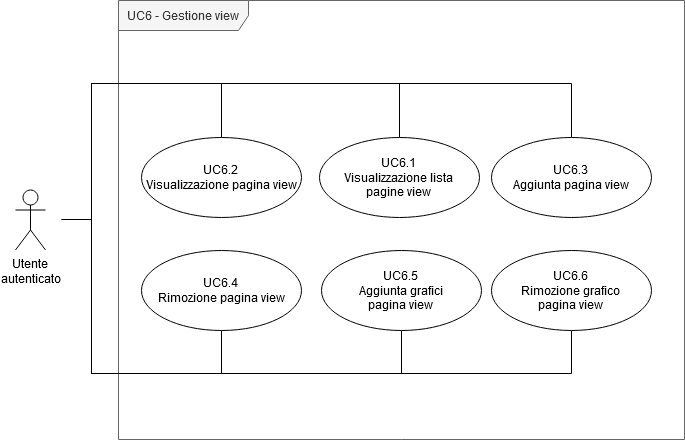
\includegraphics[scale=0.60]{res/images/uc6}
			\caption{Diagramma che riassume la gestione delle view con cui può interagire l'utente nella web app.}
		\end{figure}

		\begin{itemize}
			\item \textbf{Attori Primari}: Utente autenticato.
			\item \textbf{Descrizione}: L'utente può gestire le proprie pagine \glock{view}, attraverso cui può andare a visualizzare grafici con correlazioni sulla base dei sensori disponibili per l'ente.
			\item \textbf{Precondizione}: L'utente è autenticato e naviga all'interno delle proprie \glock{view}.
			\item \textbf{Postcondizione}: L'utente ha visualizzato o gestito le proprie \glock{view}.
			\item \textbf{Scenario Principale}:
			\begin{enumerate}
				\item{L'utente naviga all'interno delle proprie \glock{view};}
				\item{L'utente visualizza o gestisce le \glock{view} da lui create.}
			\end{enumerate}	
		\end{itemize}

			\subsubsection{UC 6.1 - Visualizzazione lista pagine view}
			\begin{itemize}
				\item \textbf{Attori Primari}: Utente autenticato.
				\item \textbf{Descrizione}: L'utente può visualizzare tutte le proprie \glock{view}.
				\item \textbf{Precondizione}: L'utente naviga all'interno delle proprie \glock{view}.
				\item \textbf{Postcondizione}: L'utente ha visualizzato le proprie \glock{view}.
				\item \textbf{Scenario Principale}:
				\begin{enumerate}
					\item{L'utente visualizza l'elenco completo delle sue pagine \glock{view}.}
				\end{enumerate}	
			\end{itemize}

			\subsubsection{UC 6.2 - Visualizzazione pagina view}
			\begin{itemize}
				\item \textbf{Attori Primari}: Utente autenticato.
				\item \textbf{Descrizione}: L'utente può aprire e visualizzare una pagina \glock{view}.
				\item \textbf{Precondizione}: L'utente naviga all'interno delle proprie \glock{view} e ha almeno una pagina \glock{view} attiva.
				\item \textbf{Postcondizione}: L'utente visualizza una pagina \glock{view} specifica.
				\item \textbf{Scenario Principale}:
				\begin{enumerate}
					\item{L'utente visualizza l'elenco completo delle sue pagine \glock{view};}
					\item{L'utente seleziona una pagina view \glock{view}.}
				\end{enumerate}	
			\end{itemize}

			\subsubsection{UC 6.3 - Aggiunta pagina view}
			\begin{itemize}
				\item \textbf{Attori Primari}: Utente autenticato.
				\item \textbf{Descrizione}: L'utente aggiunge una pagina \glock{view} attraverso un form che deve compilare.
				\item \textbf{Precondizione}: L'utente naviga all'interno delle proprie \glock{view}.
				\item \textbf{Postcondizione}: L'utente ha aggiunto una pagina \glock{view}.
				\item \textbf{Scenario Principale}:
				\begin{enumerate}
					\item{L'utente inserisce il nome della pagina view compilando un campo (UC 6.3.1);}
					\item{L'utente ha aggiunto una nuova pagina \glock{view}.}
				\end{enumerate}	
			\end{itemize}

			\paragraph{UC 6.3.1 - Inserimento nome pagina view}
			\begin{itemize}
				\item \textbf{Attori Primari}: Utente autenticato.
				\item \textbf{Descrizione}: L'utente compila un form per aggiungere una pagina \glock{view}.
				\item \textbf{Precondizione}: L'utente sta aggiungendo una nuova pagina \glock{view}.
				\item \textbf{Postcondizione}: L'utente ha compilato il nome della pagina \glock{view}.
				\item \textbf{Scenario Principale}:
				\begin{enumerate}
					\item{L'utente sta compilando il form di aggiunta pagina \glock{view};}
					\item{L'utente compila il nome della pagina \glock{view};}
					\item{L'utente ha aggiunto una nuova pagina \glock{view}.}
				\end{enumerate}	
			\end{itemize}

			\subsubsection{UC 6.4 - Eliminazione pagina view}
			\begin{itemize}
				\item \textbf{Attori Primari}: Utente autenticato.
				\item \textbf{Descrizione}: L'utente elimina una pagina \glock{view} a lui disponibile.
				\item \textbf{Precondizione}: L'utente naviga all'interno delle proprie \glock{view}.
				\item \textbf{Postcondizione}: L'utente ha eliminato una pagina \glock{view}.
				\item \textbf{Scenario Principale}:
				\begin{enumerate}
					\item L'utente seleziona una pagina \glock{view} e la rimuove;
					\item L'utente non visualizza più la pagina \glock{view} rimossa e i grafici a essa associati.
				\end{enumerate}	
			\end{itemize}

			\subsubsection{UC 6.5 - Creazione grafici view}

			\begin{figure}[H]
				\centering
				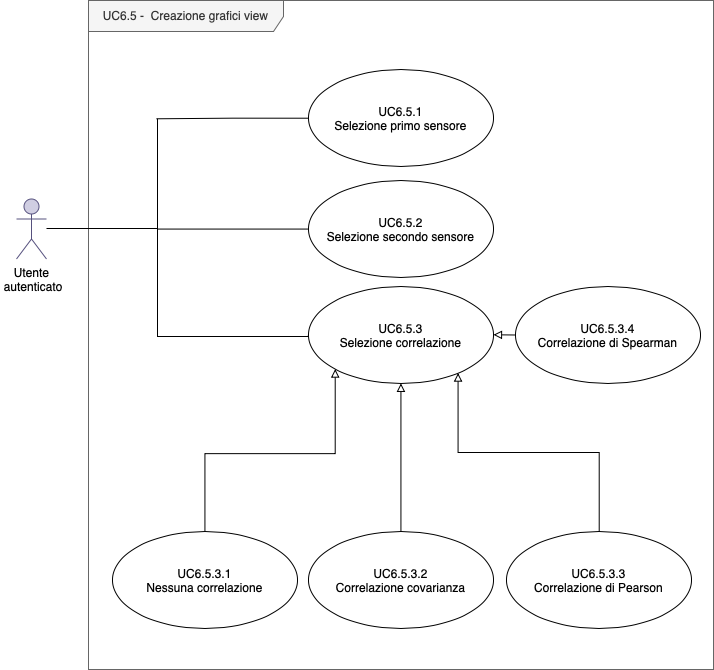
\includegraphics[scale=0.60]{res/images/uc6.5}
				\caption{Diagramma che contiene le possibili selezioni alla creazione di un grafico.}
			\end{figure}

			\begin{itemize}
				\item \textbf{Attori Primari}: Utente autenticato.
				\item \textbf{Descrizione}: L'utente può inserire un nuovo grafico all'interno di una pagina \glock{view} andando a selezionare uno o due dati da visualizzare e il tipo di correlazione tra essi.
				\item \textbf{Precondizione}: L'utente naviga all'interno di una \glock{view} che ha selezionato.
				\item \textbf{Postcondizione}: L'utente visualizza il grafico con i dati di uno o due sensori e la correlazione tra i dati
				\item \textbf{Scenario Principale}:
				\begin{enumerate}
					\item{L'utente seleziona il primo sensore di cui visualizzare i dati (UC 6.5.1);}
					\item{L'utente seleziona il secondo sensore di cui visualizzare i dati (UC 6.5.2);}
					\item{L'utente seleziona il tipo di correlazione tra i dati che intende visualizzare (UC 6.5.3);}
					\item{L'utente conferma il grafico e visualizza quanto richiesto.}
				\end{enumerate}	
			\end{itemize}

			\paragraph{UC 6.5.1 - Selezione primo sensore}
			\begin{itemize}
				\item \textbf{Attori Primari}: Utente autenticato.
				\item \textbf{Descrizione}: L'utente sta aggiungendo un nuovo grafico alla sua pagina \glock{view} e sta selezionando un dato di cui visualizzare l'andamento. Il campo è obbligatorio.
				\item \textbf{Precondizione}: L'utente sta aggiungendo una nuovo grafico a una pagina \glock{view}.
				\item \textbf{Postcondizione}: L'utente ha compilato un campo per l'aggiunta del grafico in una pagina \glock{view}.
				\item \textbf{Scenario Principale}:
				\begin{enumerate}
					\item{L'utente seleziona un sensore da cui reperire i dati da far visualizzare nel grafico.}
				\end{enumerate}	
			\end{itemize}

			\paragraph{UC 6.5.2 - Selezione secondo sensore}
			\begin{itemize}
				\item \textbf{Attori Primari}: Utente autenticato.
				\item \textbf{Descrizione}: L'utente sta aggiungendo un nuovo grafico alla sua pagina \glock{view} e sta selezionando un dato di cui visualizzare l'andamento. Il campo è opzionale.
				\item \textbf{Precondizione}: L'utente sta aggiungendo una nuovo grafico a una pagina \glock{view}.
				\item \textbf{Postcondizione}: L'utente ha compilato un campo per l'aggiunta del grafico in una pagina \glock{view}.
				\item \textbf{Scenario Principale}:
				\begin{enumerate}
					\item{L'utente seleziona un sensore da cui reperire i dati da far visualizzare nel grafico.}
				\end{enumerate}	
			\end{itemize}

			\paragraph{UC 6.5.3 - Selezione correlazione}
			\begin{itemize}
				\item \textbf{Attori Primari}: Utente autenticato.
				\item \textbf{Descrizione}: L'utente sta aggiungendo un nuovo grafico alla sua pagina \glock{view} e sta selezionando la correlazione tra i dati da visualizzare. Le correlazioni disponibili sono:
				\begin{itemize}
					\item Nessuna correlazione;
					\item Covarianza;
					\item Correlazione di Pearson;
					\item Correlazione di Spearman.
				\end{itemize}
				\item \textbf{Precondizione}: L'utente sta aggiungendo una nuovo grafico a una pagina \glock{view}.
				\item \textbf{Postcondizione}: L'utente ha compilato un campo per l'aggiunta del grafico in una pagina \glock{view}.
				\item \textbf{Scenario Principale}:
				\begin{enumerate}
					\item{L'utente seleziona la correlazione da visualizzare insieme al grafico.}
				\end{enumerate}	
			\end{itemize}

			\subparagraph{UC 6.5.3.1 - Nessuna correlazione}
			\begin{itemize}
				\item \textbf{Attori Primari}: Utente autenticato.
				\item \textbf{Descrizione}: L'utente sta aggiungendo un nuovo grafico alla sua pagina \glock{view} e ha selezionato "Nessuna correlazione". 
				\item \textbf{Precondizione}: L'utente sta aggiungendo una nuovo grafico a una pagina \glock{view}.
				\item \textbf{Postcondizione}: L'utente ha compilato un campo per l'aggiunta del grafico in una pagina \glock{view}.
				\item \textbf{Scenario Principale}:
				\begin{enumerate}
					\item{L'utente seleziona la correlazione da visualizzare insieme al grafico.}
				\end{enumerate}	
			\end{itemize}

			\subparagraph{UC 6.5.3.2 - Correlazione covarianza}
			\begin{itemize}
				\item \textbf{Attori Primari}: Utente autenticato.
				\item \textbf{Descrizione}: L'utente sta aggiungendo un nuovo grafico alla sua pagina \glock{view} e ha selezionato la correlazione covarianza. 
				\item \textbf{Precondizione}: L'utente sta aggiungendo una nuovo grafico a una pagina \glock{view}.
				\item \textbf{Postcondizione}: L'utente ha compilato un campo per l'aggiunta del grafico in una pagina \glock{view}.
				\item \textbf{Scenario Principale}:
				\begin{enumerate}
					\item{L'utente seleziona la correlazione da visualizzare insieme al grafico.}
				\end{enumerate}	
			\end{itemize}

			\subparagraph{UC 6.5.3.3 - Correlazione di Pearson}
			\begin{itemize}
				\item \textbf{Attori Primari}: Utente autenticato.
				\item \textbf{Descrizione}: L'utente sta aggiungendo un nuovo grafico alla sua pagina \glock{view} e ha selezionato correlazione di Pearson. 
				\item \textbf{Precondizione}: L'utente sta aggiungendo una nuovo grafico a una pagina \glock{view}.
				\item \textbf{Postcondizione}: L'utente ha compilato un campo per l'aggiunta del grafico in una pagina \glock{view}.
				\item \textbf{Scenario Principale}:
				\begin{enumerate}
					\item{L'utente seleziona la correlazione da visualizzare insieme al grafico.}
				\end{enumerate}	
			\end{itemize}

			\subparagraph{UC 6.5.3.4 - Correlazione di Spearman}
			\begin{itemize}
				\item \textbf{Attori Primari}: Utente autenticato.
				\item \textbf{Descrizione}: L'utente sta aggiungendo un nuovo grafico alla sua pagina \glock{view} e ha selezionato correlazione di Spearman. 
				\item \textbf{Precondizione}: L'utente sta aggiungendo una nuovo grafico a una pagina \glock{view}.
				\item \textbf{Postcondizione}: L'utente ha compilato un campo per l'aggiunta del grafico in una pagina \glock{view}.
				\item \textbf{Scenario Principale}:
				\begin{enumerate}
					\item{L'utente seleziona la correlazione da visualizzare insieme al grafico.}
				\end{enumerate}	
			\end{itemize}


			\subsubsection{UC 6.6 - Rimozione grafico pagina view}
			\begin{itemize}
				\item \textbf{Attori Primari}: Utente autenticato.
				\item \textbf{Descrizione}: L'utente può rimuovere un grafico che viene visualizzato su una pagina \glock{view}.
				\item \textbf{Precondizione}: L'utente naviga all'interno di una \glock{view} che ha selezionato e sta visualizzando almeno un grafico.
				\item \textbf{Postcondizione}: L'utente ha eliminato un grafico dalla pagina \glock{view} .
				\item \textbf{Scenario Principale}:
				\begin{enumerate}
					\item{L'utente seleziona un grafico dalla pagina \glock{view} e lo rimuove.}
					\item{L'utente non visualizza più quel grafico in quella pagina.}
				\end{enumerate}	
			\end{itemize}

		% =================
		% UC 7 - [NICE]

		\subsubsection{UC 7 - Gestione utenti ente}
		
		
		
		\begin{itemize}
			\item \textbf{Attori Primari}: [ME]
			\item \textbf{Descrizione}: Il moderatore ente gestisce gli utenti del proprio ente.
			\item \textbf{Precondizione}: Il moderatore ente seleziona la voce "Gestione utenti ente".
			\item \textbf{Postcondizione}: Il moderatore ente ha visualizzato/gestito gli utenti appartenenti al proprio ente.
			\item \textbf{Scenario Principale}:
			\begin{enumerate}
				\item{Il moderatore ente seleziona la voce "Gestione utenti ente"}
				\item{Il moderatore ente visualizza la schermata per la gestione degli utenti ente}
				\item{Il moderatore ente visualizza/gestisce gli utenti appartenenti al proprio ente}
				\item{Il moderatore ente ha visualizzato/gestito gli utente del proprio ente}
			\end{enumerate}	
		\end{itemize}
			
			\paragraph{UC 7.1 - Visualizzazione utenti ente}
			\begin{itemize}
				\item \textbf{Attori Primari}: [ME]
				\item \textbf{Descrizione}: Il moderatore ente visualizza gli utenti del proprio ente.
				\item \textbf{Precondizione}: Il moderatore ente visualizza la schermata per la gestione degli utenti ente.
				\item \textbf{Postcondizione}: Il moderatore ente ha visualizzato la lista degli utenti appartenenti al proprio ente.
				\item \textbf{Scenario Principale}:
				\begin{enumerate}
					\item{Il moderatore ente visualizza la schermata per la gestione degli utenti ente}
					\item{Il moderatore ente visualizza la lista degli utenti appartenenti al proprio ente}
					\item{Il moderatore ente ha visualizzato gli utenti del proprio ente}
				\end{enumerate}	
			\end{itemize}
			
			\paragraph{UC 7.2 - Creazione utente ente}
			\begin{itemize}
				\item \textbf{Attori Primari}: [ME]
				\item \textbf{Descrizione}: Il moderatore ente aggiunge un nuovo utente al proprio ente.
				\item \textbf{Precondizione}: Il moderatore ente visualizza la schermata per la gestione degli utenti ente.
				\item \textbf{Postcondizione}: Il moderatore ente ha aggiunto un utente al proprio ente.
				\item \textbf{Scenario Principale}:
				\begin{enumerate}
					\item{Il moderatore ente visualizza la schermata per la gestione degli utenti ente}
					\item{Il moderatore ente seleziona la voce "aggiungi utente ente"}
					\item{Il moderatore ente compila il form utente con i dati dell'utente da aggiungere}
					\item{Il moderatore ente preme sul bottone di salvataggio per aggiungere il nuovo utente}
					\item{Il moderatore ente ha aggiunto un nuovo utente appartenente al proprio ente}
				\end{enumerate}	
				\item \textbf{Inclusioni}:
					\item Il moderatore ente compila il form utente con i dati dell'utente da aggiungere (UC 7.3)
				\item \textbf{Estensioni}:
				\begin{itemize}
					\item Il moderatore ente inserisce un email non valida (UC 7.4)
					\item Il moderatore ente inserisce un nome e/o cognome non validi (UC 7.5)
				\end{itemize}
			\end{itemize}
			
			\paragraph{UC 7.3 - Compilazione form utente}
			\begin{itemize}
				\item \textbf{Attori Primari}: [ME]
				\item \textbf{Descrizione}: Il moderatore ente compila i campi per l'aggiunta/modifica dell'utente: il campo "email", corrispondente all'email dell'utente, e i campi "nome" e "cognome", corrispondenti al nominativo dell'utente.
				\item \textbf{Precondizione}: Il moderatore ente ha selezionato la voce "aggiungi utente ente" o "modifica utente ente".
				\item \textbf{Postcondizione}: Il moderatore ente ha compilato il form utente.
				\item \textbf{Scenario Principale}:
				\begin{enumerate}
					\item{Il moderatore ente seleziona la voce "aggiungi utente ente"}
					\item{Il moderatore ente compila il campo "email"}
					\item{Il moderatore ente compila il campo "nome"}
					\item{Il moderatore ente compila il campo "cognome"}
					\item{Il moderatore ente ha compilato il form utente}
				\end{enumerate}	
			\end{itemize}
			
			\paragraph{UC 7.4 - Email non valida}
			\begin{itemize}
				\item \textbf{Attori Primari}: [ME]
				\item \textbf{Descrizione}: Dopo aver premuto il bottone per salvare i dati inseriti nel form utente viene visualizzato il messaggio di errore "Email non valida" perchè l'email inserita non è valida. 
				\item \textbf{Precondizione}: Il moderatore ente ha premuto sul bottone di salvataggio del form utente.
				\item \textbf{Postcondizione}: Visualizzazione messaggio di errore "Email non valida"
				\item \textbf{Scenario Principale}:
				\begin{enumerate}
					\item{Il moderatore ente ha premuto sul bottone di salvataggio del form utente}
					\item{La email inserita nel campo "email" non è valida}
					\item{Viene visualizzato il messaggio di errore "Email non valida"}
				\end{enumerate}	
			\end{itemize}
			
			\paragraph{UC 7.5 - Nome e/o cognome non validi}
			\begin{itemize}
				\item \textbf{Attori Primari}: [ME]
				\item \textbf{Descrizione}: Dopo aver premuto il bottone per salvare i dati inseriti nel form utente viene visualizzato il messaggio di errore "Nome e/o cognome non validi" perchè il nome e/o il cognome inseriti non sono validi. 
				\item \textbf{Precondizione}: Il moderatore ente ha premuto sul bottone di salvataggio del form utente.
				\item \textbf{Postcondizione}: Visualizzazione messaggio di errore "Nome e/o cognome non validi"
				\item \textbf{Scenario Principale}:
				\begin{enumerate}
					\item{Il moderatore ente ha premuto sul bottone di salvataggio del form utente}
					\item{Il nome nel campo "nome" non è valido e/o il cognome nel campo "cognome" non è valido}
					\item{Viene visualizzato il messaggio di errore "Nome e/o cognome non validi"}
				\end{enumerate}	
			\end{itemize}
			
			\paragraph{UC 7.6 - Visualizza dati utenti ente}
			\begin{itemize}
				\item \textbf{Attori Primari}: [ME]
				\item \textbf{Descrizione}: Il moderatore ente visualizza i dati dell'utente selezionato dalla lista degli utenti del proprio ente.
				\item \textbf{Precondizione}: Il moderatore ente seleziona un utente dalla lista degli utenti del proprio ente.
				\item \textbf{Postcondizione}: Il moderatore ente ha visualizzato i dati dell'utente selezionato appartenente al proprio ente.
				\item \textbf{Scenario Principale}:
				\begin{enumerate}
					\item{Il moderatore ente seleziona un utente dalla lista degli utenti del proprio ente}
					\item{Il moderatore ente seleziona la voce "visualizza dati utente ente"}
					\item{Il moderatore ente visualizza i dati dell'utente selezionato}
					\item{Il moderatore ha visualizzato i dati dell'utente selezionato}
				\end{enumerate}
			\end{itemize}
			
			\paragraph{UC 7.7 - Modifica dati utenti ente}
			\begin{itemize}
				\item \textbf{Attori Primari}: [ME]
				\item \textbf{Descrizione}: Il moderatore ente modifica l'utente selezionato dalla lista degli utenti del proprio ente.
				\item \textbf{Precondizione}: Il moderatore ente seleziona un utente dalla lista degli utenti del proprio ente.
				\item \textbf{Postcondizione}: Il moderatore ente ha modificato l'utente selezionato appartenente al proprio ente.
				\item \textbf{Scenario Principale}:
				\begin{enumerate}
					\item{Il moderatore ente seleziona un utente dalla lista degli utenti del proprio ente}
					\item{Il moderatore seleziona la voce "modifica utente ente"}
					\item{Il moderatore compila il form utente contenente i dati da modificare dell'utente}
					\item{Il moderatore ente preme sul bottone di salvataggio per modificare l'utente selezionato}
					\item{Il moderatore ha modificato l'utente selezionato}
				\end{enumerate}	
				\item \textbf{Inclusioni}:
					\item Il moderatore compila il form utente con i dati dell'utente da modificare (UC 7.3)
				\item \textbf{Estensioni}:
				\begin{itemize}
					\item Il moderatore inserisce un email non valida (UC 7.4)
					\item Il moderatore inserisce un nome e/o cognome non validi (UC 7.5)
				\end{itemize}
			\end{itemize}
			
			\paragraph{UC 7.8 - Rimozione utenti ente}
			\begin{itemize}
				\item \textbf{Attori Primari}: [ME]
				\item \textbf{Descrizione}: Il moderatore ente rimuove dal sistema l'utente selezionato dalla lista degli utenti del proprio ente.
				\item \textbf{Precondizione}: Il moderatore ente seleziona un utente dalla lista degli utenti del proprio ente.
				\item \textbf{Postcondizione}: Il moderatore ente ha rimosso l'utente selezionato appartenente al proprio ente dal sistema.
				\item \textbf{Scenario Principale}:
				\begin{enumerate}
					\item{Il moderatore ente seleziona un utente appartenente al proprio ente da rimuovere}
					\item{Il moderatore ente seleziona la voce "Rimuovi utente ente"}
					\item{Il moderatore ente ha rimosso l'utente selezionato appartenente al proprio ente dal sistema.}
				\end{enumerate}		
			\end{itemize}


		% =================
		% UC 8 - [NICE]

			\subsection{UC 8 - Gestione alert ente}
			
		\begin{itemize}
			\item \textbf{Attori Primari}: Membro, Moderatore ente.
			\item \textbf{Descrizione}: L'utente gestisce gli \glock{alert} del proprio ente, impostande le soglie oltre il quale scatenare le notifiche per gli utenti.
			\item \textbf{Precondizione}: L'utente è autenticato e naviga all'interno della gestione \glock{alert}.
			\item \textbf{Postcondizione}: L'utente ha visualizzato o gestito gli \glock{alert} del proprio ente.
			\item \textbf{Scenario Principale}:
			\begin{enumerate}
				\item{L'utente naviga all'interno della gestione \glock{alert} del proprio ente;}
				\item{L'utente ha visualizzato o gestito gli \glock{alert} del proprio ente.}
			\end{enumerate}	
		\end{itemize}
			
			\subsubsection{UC 8.1 - Visualizzazione alert ente}
			\begin{itemize}
				\item \textbf{Attori Primari}: Membro, Moderatore ente.
				\item \textbf{Descrizione}: L'utente può visualizzare gli \glock{alert} appartenenti al proprio ente.
				\item \textbf{Precondizione}: L'utente naviga all'interno della gestione \glock{alert}.
				\item \textbf{Postcondizione}: L'utente ha visualizzato la lista degli \glock{alert} del proprio ente.
				\item \textbf{Scenario Principale}:
				\begin{enumerate}
					\item{L'utente visualizza la lista degli \glock{alert} del proprio ente.}
				\end{enumerate}	
			\end{itemize}
			
			\subsubsection{UC 8.2 - Inserimento alert ente}
			\begin{itemize}
				\item \textbf{Attori Primari}: Moderatore ente.
				\item \textbf{Descrizione}: L'utente può inserire un nuovo \glock{alert} per il proprio ente.
				\item \textbf{Precondizione}: L'utente naviga all'interno della gestione \glock{alert}.
				\item \textbf{Postcondizione}: L'utente ha inserito un nuovo \glock{alert} per gli utenti appartenenti al proprio ente.
				\item \textbf{Scenario Principale}:
				\begin{enumerate}
					\item{L'utente compila i campi con i dati dell'\glock{alert} da inserire;}
					\item L'utente seleziona un sensore tra quelli disponibile su cui eseguire il controllo (UC 8.2.1);
					\item L'utente inserisce una soglia da controllare per il sensore (UC 8.2.2);
					\item{L'utente ha inserito un nuovo \glock{alert} per gli utenti appartenenti al proprio ente.}
				\end{enumerate}
				\item \textbf{Estensioni}:
				\begin{itemize}
					\item L'utente inserisce dei valori soglia non validi (UC 8.4).
				\end{itemize}		
			\end{itemize}
			
				\paragraph{UC 8.2.1 - Selezione sensore per nuovo alert}
				\begin{itemize}
					\item \textbf{Attori Primari}: Moderatore ente.
					\item \textbf{Descrizione}: L'utente compila un campo per l'inserimento di un nuovo \glock{alert} e in particolare seleziona un sensore su cui eseguire il controllo.
					\item \textbf{Precondizione}: L'utente sta inserendo i dati per un nuovo \glock{alert}.
					\item \textbf{Postcondizione}: L'utente ha compilato il campo richiesto.
					\item \textbf{Scenario Principale}:
					\begin{enumerate}
						\item{L'utente seleziona il sensore disponibile da verificare tra un elenco di quelli disponibili.}
					\end{enumerate}	
				\end{itemize}

				\paragraph{UC 8.2.2 - Inserimento soglia per nuovo alert}
				\begin{itemize}
					\item \textbf{Attori Primari}: Moderatore ente.
					\item \textbf{Descrizione}: L'utente compila un campo per l'inserimento di un nuovo \glock{alert} e in particolare seleziona la soglia da controllare.
					\item \textbf{Precondizione}: L'utente sta inserendo i dati per un nuovo \glock{alert}.
					\item \textbf{Postcondizione}: L'utente ha compilato il campo richiesto.
					\item \textbf{Scenario Principale}:
					\begin{enumerate}
						\item{L'utente inserisce la soglia del sensore da verificare.}
					\end{enumerate}	
				\end{itemize}

			\subsubsection{UC 8.3 - Rimozione alert ente}
			\begin{itemize}
				\item \textbf{Attori Primari}: Moderatore ente.
				\item \textbf{Descrizione}: L'utente può rimuovere un \glock{alert} selezionandolo dalla lista degli \glock{alert} attivi del proprio ente.
				\item \textbf{Precondizione}: L'utente naviga all'interno della gestione \glock{alert} e ha disponibile almeno un alert.
				\item \textbf{Postcondizione}: L'utente ha rimosso l'\glock{alert} selezionato del proprio ente dal sistema.
				\item \textbf{Scenario Principale}:
				\begin{enumerate}
					\item{L'utente seleziona un \glock{alert} dalla lista degli \glock{alert} del proprio ente e lo rimuove;}
					\item{L'utente non visualizza più l'\glock{alert} selezionato.}
				\end{enumerate}	
			\end{itemize}

			\subsubsection{UC 8.4 - Errore valore soglia}
			\begin{itemize}
				\item \textbf{Attori Primari}: Moderatore ente.
				\item \textbf{Descrizione}: Dopo aver premuto il bottone per confermare i campi inseriti, viene visualizzato il messaggio di errore che segnala un valore soglia non valido.
				\item \textbf{Precondizione}: L'utente ha inserito i campi richiesti e il sistema sta elaborando la richiesta.
				\item \textbf{Postcondizione}: Visualizzazione messaggio di errore specifico.
				\item \textbf{Scenario Principale}:
				\begin{enumerate}
					\item{Il sistema elabora la richiesta;}
					\item{Viene visualizzato il messaggio di errore che spiega che il valore soglia inserito per un \glock{alert} non è valido. }
				\end{enumerate}
			\end{itemize}
			
			\subsubsection{UC 8.5 - Modifica alert ente}
			\begin{itemize}
				\item \textbf{Attori Primari}: Moderatore ente.
				\item \textbf{Descrizione}: L'utente può modificare \glock{alert} esistente per il proprio ente.
				\item \textbf{Precondizione}: L'utente naviga all'interno della gestione \glock{alert}.
				\item \textbf{Postcondizione}: L'utente ha inserito un nuovo \glock{alert} per gli utenti appartenenti al proprio ente.
				\item \textbf{Scenario Principale}:
				\begin{enumerate}
					\item{L'utente compila i campi con i dati dell'\glock{alert} da inserire;}
					\item L'utente modifica la soglia da controllare per il sensore (UC 8.5.1);
					\item{L'utente ha inserito un nuovo \glock{alert} per gli utenti appartenenti al proprio ente.}
				\end{enumerate}
				\item \textbf{Estensioni}:
				\begin{itemize}
					\item L'utente inserisce dei valori soglia non validi (UC 8.4).
				\end{itemize}		
			\end{itemize}

				\paragraph{UC 8.5.1 - Modifica soglia per alert}
				\begin{itemize}
					\item \textbf{Attori Primari}: Moderatore ente.
					\item \textbf{Descrizione}: L'utente compila un campo per la modifica di un \glock{alert} e in particolare inserisce la soglia da controllare.
					\item \textbf{Precondizione}: L'utente sta inserendo i dati per modificare un \glock{alert}.
					\item \textbf{Postcondizione}: L'utente ha compilato il campo richiesto.
					\item \textbf{Scenario Principale}:
					\begin{enumerate}
						\item{L'utente inserisce la soglia del sensore da verificare.}
					\end{enumerate}	
				\end{itemize}

		% =================
		% UC 9 - [NICE]

		\subsection{UC 9 - Ente - Visualizzazione logs membri}
		\begin{itemize}
			\item \textbf{Attori Primari}: Moderatore ente.
			\item \textbf{Descrizione}: Il moderatore ente intende visualizzare gli accessi e i movimenti effettuati dai membri appartenenti al proprio ente.
			\item \textbf{Precondizione}: L'utente è autenticato e fa parte di un ente in qualità di moderatore ente.
			\item \textbf{Postcondizione}: L'utente visualizza i logs relativi agli utenti appartenenti al proprio ente.
			\item \textbf{Scenario Principale}:
			\begin{enumerate}
				\item Nella web app, l'utente può navigare per giungere alla visualizzazione logs dei membri del proprio ente.
			\end{enumerate}	
		\end{itemize}

		% =================
		% UC 10 - [NICE]

		\subsection{UC 10 - Amministrazione - Gestione enti}

		\begin{figure}[H]
			\centering
			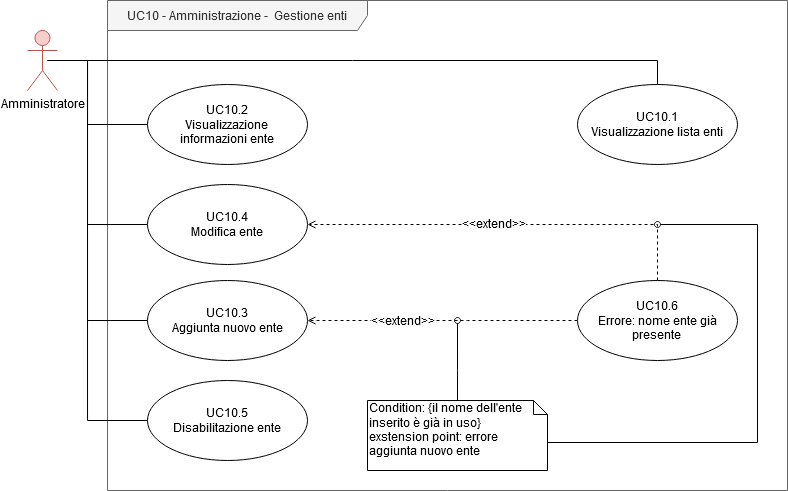
\includegraphics[scale=0.60]{res/images/uc10}
			\caption{Diagramma che descrive la gestione degli enti a livello amministrativo.}
		\end{figure}

		\begin{itemize}
			\item \textbf{attori primari:} Amministratore;
			\item \textbf{descrizione:} l'utente può gestire gli enti del sistema, visualizzando la lista completa, aggiungendone di nuovi, modificandone di esistenti e rimuovendone all'occorrenza;
			\item \textbf{precondizione:} l'utente naviga nella gestione enti per l'amministrazione;
			\item \textbf{postcondizionetcondizione:} l'utente ha visualizzato o gestito gli enti all'interno del sistema;
			\item \textbf{scenario principale:}
			\begin{enumerate}
				\item{l'utente visualizza o gestisce gli enti all'interno del sistema.}
			\end{enumerate}	
		\end{itemize}

			\subsubsection{UC 10.1 - Visualizzazione lista enti }
			\begin{itemize}
				\item \textbf{attori primari:} Amministratore;
				\item \textbf{descrizione:} l'utente può visualizzare una lista con nome e luogo della sede degli enti attivi censiti nel sistema;
				\item \textbf{precondizione:} l'utente naviga nella gestione enti per l'amministrazione;
				\item \textbf{postcondizione:} l'utente ha visualizzato la lista degli enti presenti nel sistema;
				\item \textbf{scenario principale:}
				\begin{enumerate}
					\item{l'utente visualizza la lista enti attualmente attivi e disponibili.}
				\end{enumerate}	
			\end{itemize}

			\subsubsection{UC 10.2 - Visualizzazione informazioni ente}
			\begin{itemize}
				\item \textbf{attori primari:} Amministratore;
				\item \textbf{descrizione:} l'utente può visualizzare le informazioni riguardanti uno specifico ente, quali il suo nome, il luogo della sede ed una lista con nome, cognome e mail degli utenti appartenenti a quell'ente;
				\item \textbf{precondizione:} l'utente naviga nella gestione enti per l'amministrazione;
				\item \textbf{postcondizione:} l'utente visualizza le informazioni di un ente selezionato;
				\item \textbf{scenario principale:}
				\begin{enumerate}
					\item{l'utente seleziona dalla lista un ente;}
					\item{l'utente visualizza le informazioni riguardanti l'utente selezionato.}
				\end{enumerate}	
			\end{itemize}

			\subsubsection{UC 10.3 - Aggiunta nuovo ente}
			\begin{itemize}
				\item \textbf{attori primari:} Amministratore;
				\item \textbf{descrizione:} l'utente può aggiungere un nuovo ente al sistema, inserendo le apposite informazioni richieste;
				\item \textbf{precondizione:} l'utente naviga nella gestione enti per l'amministrazione;
				\item \textbf{postcondizione:} l'utente ha creato un nuovo ente;
				\item \textbf{scenario principale:}
				\begin{enumerate}
					\item{l'utente deve compilare dei campi per proseguire con l'inserimento di un nuovo ente;}
					\item l'utente inserisce il nome ente (UC 10.3.1);
					\item l'utente inserisce la sede (luogo) in cui risiede l'ente (UC 10.3.2);
					\item{l'ente viene creato dall'utente con le informazioni fornite;}
				\end{enumerate}	
				\item \textbf{estensioni:}
					\begin{itemize}
						\item Errore: il nome ente inserito è già presente (UC 10.6).
					\end{itemize}
			\end{itemize}	

				\paragraph{UC 10.3.1 - Inserimento nome ente}
				\begin{itemize}
					\item \textbf{attori primari:} Amministratore;
					\item \textbf{descrizione:} l'utente sta aggiungendo un nuovo ente al sistema e deve compilare il campo per il nome dell'ente;
					\item \textbf{precondizione:} l'utente sta aggiungendo un nuovo ente e deve compilare un campo specifico;
					\item \textbf{postcondizione:} l'utente ha compilato il campo specifico;
					\item \textbf{scenario principale:}
					\begin{enumerate}
						\item l'utente inserisce il nome ente.
					\end{enumerate}	
				\end{itemize}	

				\paragraph{UC 10.3.2 - Inserimento della sede}
				\begin{itemize}
					\item \textbf{attori primari:} Amministratore;
					\item \textbf{descrizione:} l'utente sta aggiungendo un nuovo ente al sistema e deve compilare il campo per la sede dell'ente;
					\item \textbf{precondizione:} l'utente sta aggiungendo un nuovo ente e deve compilare un campo specifico;
					\item \textbf{postcondizione:} l'utente ha compilato il campo specifico;
					\item \textbf{scenario principale:}
					\begin{enumerate}
						\item l'utente inserisce la sede in cui risiede l'ente.
					\end{enumerate}	
				\end{itemize}			

			\subsubsection{UC 10.4 - Modifica ente}
			\begin{itemize}
				\item \textbf{attori primari:} Amministratore;
				\item \textbf{descrizione:} l'utente può modificare un ente esistente nel sistema, inserendo le apposite informazioni richieste;
				\item \textbf{precondizione:} l'utente naviga nella gestione enti per l'amministrazione;
				\item \textbf{postcondizione:} l'utente ha modificato l'ente che aveva selezionato;
				\item \textbf{scenario principale:}
				\begin{enumerate}
					\item l'utente seleziona un ente specifico da quelli disponibili;
					\item{l'utente deve compilare dei campi per proseguire con la modifica di un ente esistente;}
					\item l'utente modifica il nome ente (UC 10.4.1);
					\item l'utente modifica la sede (luogo) in cui risiede l'ente (UC 10.4.2);
					\item{l'ente viene creato dall'utente con le informazioni fornite;}
				\end{enumerate}	
				\item \textbf{estensioni:}
					\begin{itemize}
						\item Errore: il nome ente inserito è già presente (UC 10.6).
					\end{itemize}
			\end{itemize}	

				\paragraph{UC 10.4.1 - Modifica nome ente}
				\begin{itemize}
					\item \textbf{attori primari:} Amministratore;
					\item \textbf{descrizione:} l'utente sta modificando un ente presente nel sistema e deve compilare il campo per il nome dell'ente;
					\item \textbf{precondizione:} l'utente sta modificando un ente e deve compilare un campo specifico;
					\item \textbf{postcondizione:} l'utente ha compilato il campo specifico;
					\item \textbf{scenario principale:}
					\begin{enumerate}
						\item l'utente modifica il nome ente.
					\end{enumerate}	
				\end{itemize}	

				\paragraph{UC 10.4.2 - Modifica della sede}
				\begin{itemize}
					\item \textbf{attori primari:} Amministratore;
					\item \textbf{descrizione:} l'utente sta modificando un ente presente nel sistema e deve compilare il campo per la sede dell'ente;
					\item \textbf{precondizione:} l'utente sta modificando un ente e deve compilare un campo specifico;
					\item \textbf{postcondizione:} l'utente ha compilato il campo specifico;
					\item \textbf{scenario principale:}
					\begin{enumerate}
						\item l'utente modifica la sede in cui risiede l'ente.
					\end{enumerate}	
				\end{itemize}	


			\subsubsection{UC 10.5 - Disabilitazione ente}
			\begin{itemize}
				\item \textbf{attori primari:} Amministratore;
				\item \textbf{descrizione:} l'utente può disabilitare un ente dal sistema dal sistema;
				\item \textbf{precondizione:} l'utente visualizza la lista degli enti appartenenti al sistema;
				\item \textbf{postcondizione:} l'utente ha disabilitato l'ente selezionato;
				\item \textbf{scenario principale:}
				\begin{enumerate}
					\item{l'utente seleziona l'ente da disabilitare;}
					\item{l'utente non visualizza più l'ente selezionato.}
				\end{enumerate}	
			\end{itemize}	

			\subsubsection{UC 10.6 - Errore: nome ente già presente}
			\begin{itemize}
				\item \textbf{attori primari:} Amministratore;
				\item \textbf{descrizione:} l'utente, dopo aver compilando il campo per il nome di un ente, visualizza un errore che segnala che il nome ente è già censito nel sistema;
				\item \textbf{precondizione:} l'utente ha compilato il nome dell'ente;
				\item \textbf{postcondizione:} l'utente visualizza un errore specifico e non porta a termine l'azione intrapresa;
				\item \textbf{scenario principale:}
				\begin{enumerate}
					\item{l'utente conferma i campi compilati, tra cui quello per il nome ente;}
					\item{viene visualizzato un errore che segnala la presenza all'interno del sistema di un ente con lo stesso nome.}
				\end{enumerate}	
			\end{itemize}			


		% =================
		% UC 11 - [NICE]

		\subsection{UC 11 - Amministrazione - Gestione utenti}

		\begin{figure}[H]
			\centering
			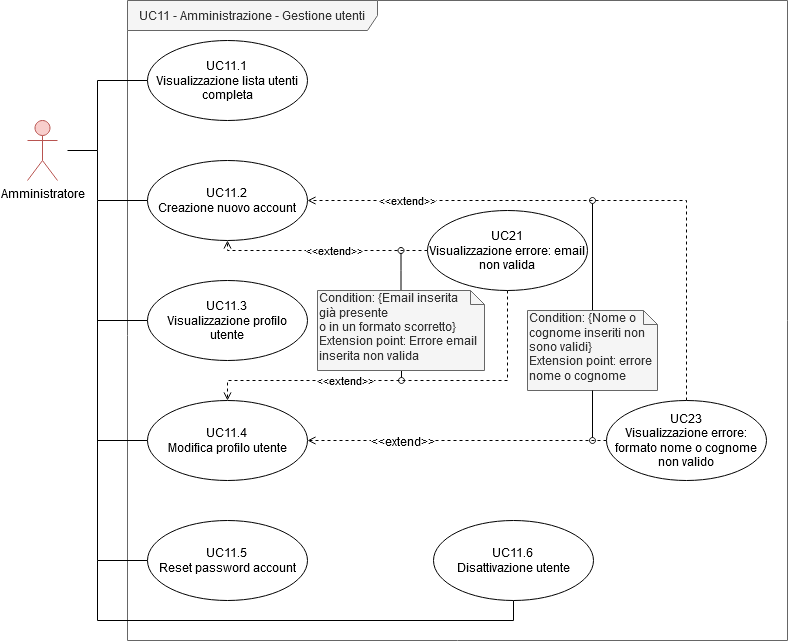
\includegraphics[scale=0.60]{res/images/uc11}
			\caption{Diagramma che descrive la gestione utenti a livello amministrativo.}
		\end{figure}

		\begin{itemize}
			\item \textbf{Attori Primari}: Amministratore.
			\item \textbf{Descrizione}: L'utente può navigare nell'area gestionale di tutti gli utenti del sistema. Può visualizzare e gestire questi utenti. 
			\item \textbf{Precondizione}: L'utente risulta autenticato nella web app e naviga nella gestione utenti per amministratori.
			\item \textbf{Postcondizione}: L'utente ha visualizzato o gestito gli utenti all'interno del sistema. 
			\item \textbf{Scenario Principale}:
			\begin{enumerate}
				\item{L'utente visualizza o gestisce gli utenti censiti dal sistema}
			\end{enumerate}	
		\end{itemize}

			\subsubsection{UC 11.1 - Visualizzazione lista utenti completa}
			\begin{itemize}
				\item \textbf{Attori Primari}: Amministratore.
				\item \textbf{Descrizione}: L'utente può visualizzare una lista con nome, cognome, mail ed ente di appartenenza di tutti gli utenti censiti nel sistema.
				\item \textbf{Precondizione}: L'utente naviga nella gestione utenti per amministratori.
				\item \textbf{Postcondizione}: L'utente visualizza la lista degli utenti registrati al sistema.
				\item \textbf{Scenario Principale}:
				\begin{enumerate}
					\item{L'utente visualizza la lista degli utenti registrati al sistema}
				\end{enumerate}	
			\end{itemize}
			
			\subsubsection{UC 11.2 - Creazione nuovo account}
			\begin{itemize}
				\item \textbf{Attori Primari}: Amministratore.
				\item \textbf{Descrizione}: L'utente può creare un nuovo account che viene inserito nel sistema e assegnato a un ente.
				\item \textbf{Precondizione}: L'utente naviga nella gestione utenti per amministratori.
				\item \textbf{Postcondizione}: L'utente ha creato un nuovo account.
				\item \textbf{Scenario Principale}:
				\begin{enumerate}
					\item{L'utente deve compilare dei campi con i dati dell'utente da aggiungere;}
					\item{L'utente compila il campo per la email;}
					\item{L'utente compila il campo per il nome;}
					\item{L'utente compila il campo per il cognome;}
					\item{L'utente seleziona l'ente a cui assegnare il nuovo account tra quelli disponibili;}
					\item{L'utente seleziona la tipologia di utente;}
					\item{L'utente ha aggiunto un nuovo utente al sistema.}
				\end{enumerate}	
				\item \textbf{Estensioni}:
				\begin{itemize}
					\item L'utente inserisce un email non valida (UC 21)
					\item L'utente inserisce un nome o cognome non validi (UC 23)
				\end{itemize}
			\end{itemize}
			
			\paragraph{UC 11.2.1 - Inserimento email}
			\begin{itemize}
				\item \textbf{Attori Primari}: Amministratore.
				\item \textbf{Descrizione}: L'utente sta creando un nuovo account che verrà inserito nel sistema e deve compilare un campo per la email. Il campo è obbligatorio.
				\item \textbf{Precondizione}: L'utente sta compilando i campi richiesti per l'aggiunta di un nuovo utente.
				\item \textbf{Postcondizione}: L'utente ha compilato il campo richiesto.
				\item \textbf{Scenario Principale}:
				\begin{enumerate}
					\item{L'utente compila il campo per la email;}
				\end{enumerate}	
			\end{itemize}

			\paragraph{UC 11.2.2 - Inserimento nome}
			\begin{itemize}
				\item \textbf{Attori Primari}: Amministratore.
				\item \textbf{Descrizione}: L'utente sta creando un nuovo account che verrà inserito nel sistema e deve compilare un campo per il nome. Il campo è obbligatorio.
				\item \textbf{Precondizione}: L'utente sta compilando i campi richiesti per l'aggiunta di un nuovo utente.
				\item \textbf{Postcondizione}: L'utente ha compilato il campo richiesto.
				\item \textbf{Scenario Principale}:
				\begin{enumerate}
					\item{L'utente compila il campo per il nome;}
				\end{enumerate}	
			\end{itemize}

			\paragraph{UC 11.2.3 - Inserimento cognome}
			\begin{itemize}
				\item \textbf{Attori Primari}: Amministratore.
				\item \textbf{Descrizione}: L'utente sta creando un nuovo account che verrà inserito nel sistema e deve compilare un campo per il cognome. Il campo è obbligatorio.
				\item \textbf{Precondizione}: L'utente sta compilando i campi richiesti per l'aggiunta di un nuovo utente.
				\item \textbf{Postcondizione}: L'utente ha compilato il campo richiesto.
				\item \textbf{Scenario Principale}:
				\begin{enumerate}
					\item{L'utente compila il campo per il cognome;}
				\end{enumerate}	
			\end{itemize}

			\paragraph{UC 11.2.4 - Selezione ente per il nuovo utente}
			\begin{itemize}
				\item \textbf{Attori Primari}: Amministratore.
				\item \textbf{Descrizione}: L'utente sta creando un nuovo account che verrà inserito nel sistema e deve compilare un campo che richiede a quale ente assegnare l'utente, tra quelli disponibili. Il campo è obbligatorio.
				\item \textbf{Precondizione}: L'utente sta compilando i campi richiesti per l'aggiunta di un nuovo utente.
				\item \textbf{Postcondizione}: L'utente ha compilato il campo richiesto.
				\item \textbf{Scenario Principale}:
				\begin{enumerate}
					\item{L'utente seleziona l'ente a cui assegnare il nuovo account tra quelli disponibili;}
				\end{enumerate}	
			\end{itemize}

			\paragraph{UC 11.2.5 - Selezione tipologia utente}
			\begin{itemize}
				\item \textbf{Attori Primari}: Amministratore.
				\item \textbf{Descrizione}: L'utente sta creando un nuovo account che verrà inserito nel sistema e deve compilare un campo che richiede a quale tipologia assegnare l'utente. Il campo è obbligatorio. Le tipologie disponibili sono:
				\begin{itemize}
					\item Membro;
					\item Moderatore ente.
				\end{itemize}
				\item \textbf{Precondizione}: L'utente sta compilando i campi richiesti per l'aggiunta di un nuovo utente.
				\item \textbf{Postcondizione}: L'utente ha compilato il campo richiesto.
				\item \textbf{Scenario Principale}:
				\begin{enumerate}
					\item{L'utente seleziona la tipologia di utente per il nuovo account;}
				\end{enumerate}	
			\end{itemize}

			\subsubsection{UC 11.3 - Visualizzazione profilo utente}
			\begin{itemize}
				\item \textbf{Attori Primari}: Amministratore.
				\item \textbf{Descrizione}: L'utente vuole visualizzare le informazioni del profilo di un utente presente nel sistema, quali: nome, cognome, username Telegram (se presente), opzione di autenticazione a due fattori (attiva o meno) ed ente di appartenenza.
				\item \textbf{Precondizione}: L'utente naviga all'interno della gestione utenti.
				\item \textbf{Postcondizione}: L'utente ha visualizzato le informazioni dell'utente selezionato.
				\item \textbf{Scenario Principale}:
				\begin{enumerate}
					\item{L'utente seleziona un utente dalla lista degli utenti;}
					\item{L'utente visualizza le informazioni dell'utente selezionato.}
				\end{enumerate}
			\end{itemize}


			\subsubsection{UC 11.4 - Modifica profilo utente}
			\begin{itemize}
				\item \textbf{Attori Primari}: Amministratore.
				\item \textbf{Descrizione}: L'utente modifica il profilo dell'utente selezionato dalla lista degli utenti.
				\item \textbf{Precondizione}: L'utente naviga all'interno della gestione utenti.
				\item \textbf{Postcondizione}: L'utente ha modificato l'utente selezionato.
				\item \textbf{Scenario Principale}:
				\begin{enumerate}
					\item L'utente seleziona un account utente che vuole modificare;
					\item L'utente deve compilare alcuni campi per proseguire nella modifica dell'utente selezionato;
					\item{L'utente modifica il campo per la email (UC 11.4.1);}
					\item{L'utente modifica il campo per il nome (UC 11.4.2);}
					\item{L'utente modifica il campo per il cognome (UC 11.4.3);}
					\item{L'utente modifica il campo Username \glock{Telegram} (UC 11.4.4);}
					\item{L'utente seleziona l'ente a cui assegnare il nuovo account tra quelli disponibili (UC 11.4.5);}
					\item{L'utente seleziona la tipologia di utente (UC 11.4.6);}
					\item{L'utente seleziona la preferenza per l'autenticazione a due fattori di quell'account (UC 11.4.7);}
					\item{L'utente ha compilato tutti i campi e conferma.}
				\end{enumerate}	
				\item \textbf{Estensioni}:
				\begin{itemize}
					\item L'utente inserisce una email non valida (UC 21);
					\item L'utente inserisce un nome o cognome non validi (UC 23).
				\end{itemize}
			\end{itemize}
			
				\paragraph{UC 11.4.1 - Modifica email}
				\begin{itemize}
					\item \textbf{Attori Primari}: Amministratore.
					\item \textbf{Descrizione}: L'utente sta modificando un account esistente censito a sistema e deve compilare un campo per la email. Il campo è obbligatorio.
					\item \textbf{Precondizione}: L'utente sta compilando i campi richiesti per la modifica di un utente.
					\item \textbf{Postcondizione}: L'utente ha compilato il campo richiesto.
					\item \textbf{Scenario Principale}:
					\begin{enumerate}
						\item{L'utente compila il campo per la email.}
					\end{enumerate}	
				\end{itemize}

				\paragraph{UC 11.4.2 - Modifica nome}
				\begin{itemize}
					\item \textbf{Attori Primari}: Amministratore.
					\item \textbf{Descrizione}: L'utente sta modificando un account esistente censito a sistema e deve compilare un campo per il nome. Il campo è obbligatorio.
					\item \textbf{Precondizione}: L'utente sta compilando i campi richiesti per la modifica di un utente.
					\item \textbf{Postcondizione}: L'utente ha compilato il campo richiesto.
					\item \textbf{Scenario Principale}:
					\begin{enumerate}
						\item{L'utente compila il campo per il nome.}
					\end{enumerate}	
				\end{itemize}

				\paragraph{UC 11.4.3 - Modifica cognome}
				\begin{itemize}
					\item \textbf{Attori Primari}: Amministratore.
					\item \textbf{Descrizione}: L'utente sta modificando un account esistente censito a sistema e deve compilare un campo per il cognome. Il campo è obbligatorio.
					\item \textbf{Precondizione}: L'utente sta compilando i campi richiesti per la modifica di un utente.
					\item \textbf{Postcondizione}: L'utente ha compilato il campo richiesto.
					\item \textbf{Scenario Principale}:
					\begin{enumerate}
						\item{L'utente compila il campo per il cognome.}
					\end{enumerate}	
				\end{itemize}

				\paragraph{UC 11.4.4 - Modifica username Telegram}
				\begin{itemize}
					\item \textbf{Attori Primari}: Amministratore.
					\item \textbf{Descrizione}: L'utente sta modificando un account esistente censito a sistema e deve compilare un campo per lo username \glock{Telegram}. Il campo è obbligatorio.
					\item \textbf{Precondizione}: L'utente sta compilando i campi richiesti per la modifica di un utente.
					\item \textbf{Postcondizione}: L'utente ha compilato il campo richiesto.
					\item \textbf{Scenario Principale}:
					\begin{enumerate}
						\item{L'utente compila il campo per lo username \glock{Telegram}.}
					\end{enumerate}	
				\end{itemize}

				\paragraph{UC 11.4.5 - Modifica ente di appartenenza}
				\begin{itemize}
					\item \textbf{Attori Primari}: Amministratore.
					\item \textbf{Descrizione}: L'utente sta modificando un account esistente censito a sistema e deve compilare un campo per assegnare quell'utente a uno degli enti censiti da sistema. Il campo è obbligatorio.
					\item \textbf{Precondizione}: L'utente sta compilando i campi richiesti per la modifica di un utente.
					\item \textbf{Postcondizione}: L'utente ha compilato il campo richiesto.
					\item \textbf{Scenario Principale}:
					\begin{enumerate}
						\item{L'utente seleziona l'ente a cui assegnare il nuovo account tra quelli disponibili.}
					\end{enumerate}	
				\end{itemize}

				\paragraph{UC 11.4.6 - Modifica tipologia di utente}
				\begin{itemize}
					\item \textbf{Attori Primari}: Amministratore.
					\item \textbf{Descrizione}: L'utente sta modificando un account esistente censito a sistema e deve compilare un campo per assegnare la tipologia di account per un dato utente. Il campo è obbligatorio. Le tipologie disponibili sono:
					\begin{itemize}
						\item Membro;
						\item Moderatore ente.
					\end{itemize}
					\item \textbf{Precondizione}: L'utente sta compilando i campi richiesti per la modifica di un utente.
					\item \textbf{Postcondizione}: L'utente ha compilato il campo richiesto.
					\item \textbf{Scenario Principale}:
					\begin{enumerate}
						\item{L'utente seleziona la tipologia di account da assegnare per un utente in base a quelli disponibili.}
					\end{enumerate}	
				\end{itemize}

				\paragraph{UC 11.4.7 - Modifica preferenza per l'autenticazione a due fattori}
				\begin{itemize}
					\item \textbf{Attori Primari}: Amministratore.
					\item \textbf{Descrizione}: L'utente sta modificando un account esistente censito a sistema e deve compilare un campo per la preferenza di attivazione dell'autenticazione a due fattori con \glock{Telegram}. Il campo è obbligatorio. Le preferenze disponibili sono:
					\begin{itemize}
						\item Abilitata;
						\item Disabilitata.
					\end{itemize}
					\item \textbf{Precondizione}: L'utente sta compilando i campi richiesti per la modifica di un utente.
					\item \textbf{Postcondizione}: L'utente ha compilato il campo richiesto.
					\item \textbf{Scenario Principale}:
					\begin{enumerate}
						\item{L'utente seleziona la preferenza per l'autenticazione a due fattori.}
					\end{enumerate}	
				\end{itemize}



			\subsubsection{UC 11.5 - Reset password account}
			\begin{itemize}
				\item \textbf{Attori Primari}: Amministratore.
				\item \textbf{Descrizione}: L'utente vuole resettare la password di un account utente censito nel sistema.
				\item \textbf{Precondizione}: L'utente naviga all'interno della gestione utenti per l'amministrazione.
				\item \textbf{Postcondizione}: L'utente ha resettato la password dell'account selezionato.
				\item \textbf{Scenario Principale}:
				\begin{enumerate}
					\item{L'utente seleziona un utente diverso tra quelli disponibili cui vuole resettare la password;}
					\item{L'utente ha resettato la password all'utente di sistema.}
				\end{enumerate}		
			\end{itemize}

			
			\subsubsection{UC 11.6 - Disattivazione utente}
			\begin{itemize}
				\item \textbf{Attori Primari}: Amministratore.
				\item \textbf{Descrizione}: L'utente vuole disattivare l'account di un utente attualmente attivo.
				\item \textbf{Precondizione}: L'utente naviga all'interno della gestione utenti per l'amministrazione.
				\item \textbf{Postcondizione}: L'utente ha disattivato l'account dell'utente selezionato.
				\item \textbf{Scenario Principale}:
				\begin{enumerate}
					\item{L'utente seleziona un utente tra quelli disponibili da disattivare;}
					\item{L'utente ha disattivato l'utente dal sistema.}
				\end{enumerate}		
			\end{itemize}

			
			


		% =================
		% UC 12 - [NICE]

			\subsection{UC 12 - Amministrazione - Gestione \glock{alert}}

		\begin{itemize}
			\item \textbf{Attori Primari}: Amministratore.
			\item \textbf{Descrizione}: L'utente navigando nella gestione degli \glock{alert} impostati dagli enti all'interno del sistema.
			\item \textbf{Precondizione}: L'utente è autenticato nella web app.
			\item \textbf{Postcondizione}: L'utente ha visualizzato o gestito gli \glock{alert} all'interno del sistema.
			\item \textbf{Scenario Principale}:
			\begin{enumerate}
				\item{L'utente, navigando nella gestione \glock{alert}, ha visualizzato o gestito gli \glock{alert} impostati dagli enti all'interno del sistema}
			\end{enumerate}	
		\end{itemize}

		\subsubsection{UC 12.1 - Visualizzazione lista completa degli \glock{alert} attivi}
		\begin{itemize}
			\item \textbf{Attori Primari}: Amministratore.
			\item \textbf{Descrizione}: L'utente vuole visualizzare la lista degli \glock{alert} per tutti gli enti attivi nel sistema.
			\item \textbf{Precondizione}: L'utente sta navigando all'interno della gestione \glock{alert}.
			\item \textbf{Postcondizione}: L'utente sta visualizzando gli \glock{alert} presenti nel sistema.
			\item \textbf{Scenario Principale}:
			\begin{enumerate}
				\item{L'utente visualizza la lista degli \glock{alert} attivi nel sistema.}
			\end{enumerate}	
		\end{itemize}

		\subsubsection{UC 12.2 - Rimozione singolo \glock{alert}}
		\begin{itemize}
			\item \textbf{Attori Primari}: Amministratore.
			\item \textbf{Descrizione}: L'utente vuole rimuovere un qualsiasi \glock{alert} dalla lista degli \glock{alert} attivi.
			\item \textbf{Precondizione}: L'utente sta navigando all'interno della gestione \glock{alert} e visualizza almeno un \glock{alert}
			\item \textbf{Postcondizione}: L'utente ha rimosso dal sistema l'\glock{alert} selezionato.
			\item \textbf{Scenario Principale}:
			\begin{enumerate}
				\item{L'utente seleziona un \glock{alert} dalla lista degli \glock{alert} e lo rimuove;}
				\item{L'utente non visualizza più l'\glock{alert} precedentemente selezionato.}
			\end{enumerate}	
		\end{itemize}

		% =================
		% UC 13 - [NICE]

		\subsection{UC 13 - Amministrazione - Visualizzazione logs utenti}
		\begin{itemize}
			\item \textbf{Attori Primari}: Amministratore.
			\item \textbf{Descrizione}: L'amministratore vuole visualizzare gli accessi e i movimenti degli utenti presenti all'interno del sistema.
			\item \textbf{Precondizione}: L'utente è autenticato in qualità di amministratore.
			\item \textbf{Postcondizione}: L'utente visualizza la lista delle logs di tutti gli utenti del sistema.
			\item \textbf{Scenario Principale}:
			\begin{enumerate}
				\item Nella web app, l'utente può navigare per giungere alla visualizzazione logs utenti.
			\end{enumerate}	
		\end{itemize}
		

		\subsection{Contesto riassuntivo per le interazioni con Telegram}

		\begin{figure}[H]
			\centering
			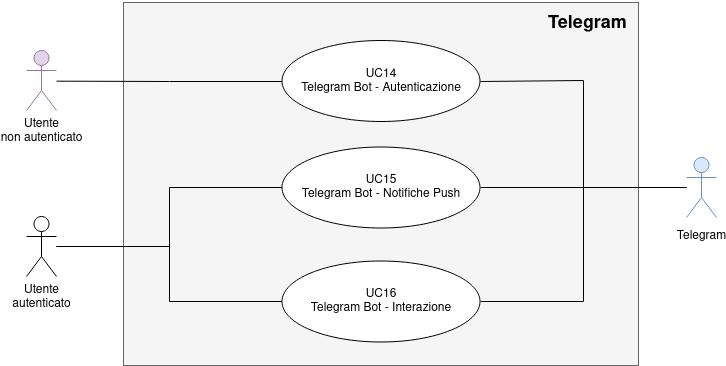
\includegraphics[scale=0.6]{res/images/telegram}
			\caption{Diagramma riassuntivo che illustra le interazioni principali con Telegram.}
		\end{figure}

		% =================
		% UC 14 - [NICE] 

		\subsection{UC 14 - Telegram - Autenticazione}

	\begin{figure}[H]
		\centering
		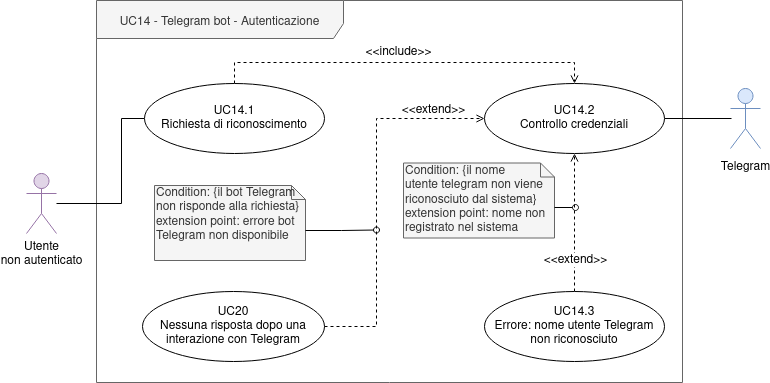
\includegraphics[scale=0.60]{res/images/uc14}
		\caption{Diagramma che descrive il processo di autenticazione tramite Telegram.}
	\end{figure}

	\begin{itemize}
		\item \textbf{attori primari:} utente non autenticato;
		\item \textbf{attori secondari:} \glock{Telegram};
		\item \textbf{descrizione:} l'utente tenta di autenticarsi con il \glock{bot} \glock{Telegram}, per farlo entra all'interno dell'applicazione e inizia la chat con il \glock{bot}. Attraverso \glock{Telegram}, viene segnalato al \glock{bot} il nome utente e il \glock{bot} verifica se questo è censito all'interno del sistema. Se viene riconosciuto, viene registrata l'apertura e l'autenticazione del canale di comunicazione tra il \glock{bot} e l'utente, diventando quest'ultimo autenticato;
		\item \textbf{precondizione:} l'utente è nell'applicazione di \glock{Telegram} e non ha una chat autenticata con il \glock{bot};
		\item \textbf{postcondizione:} l'utente effettua l'autenticazione e il canale di comunicazione tra utente e \glock{bot} viene salvato nel sistema;
		\item \textbf{scenario principale:}
		\begin{enumerate}
			\item l'utente seleziona nell'applicazione di \glock{Telegram} il \glock{bot} di sistema dal pannello di ricerca;
			\item l'utente tenta di aprire una conversazione con il \glock{bot};
			\item l'utente viene autenticato e la chat viene salvata nel sistema.
		\end{enumerate}
	\end{itemize}

	\subsubsection{UC 14.1 - Richiesta di riconoscimento}

	\begin{itemize}
		\item \textbf{attori primari:} utente non autenticato;
		\item \textbf{descrizione:} l'utente invia una richiesta al \glock{bot} di volersi autenticare per poter aprire il canale di comunicazione;
		\item \textbf{precondizione:} l'utente è nell'applicazione di \glock{Telegram} e non ha una chat autenticata con il \glock{bot};
		\item \textbf{postcondizione:} l'utente invia il comando per richiedere l'autenticazione;
		\item \textbf{scenario principale:}
		\begin{enumerate}
			\item l'utente seleziona nell'applicazione di \glock{Telegram} il \glock{bot} del sistema;
			\item l'utente tenta di aprire una conversazione con il \glock{bot};
			\item per attivare la conversazione con il \glock{bot} ed autenticarsi, l'utente invia il comando predefinito;
		\end{enumerate}
		\item \textbf{inclusioni:}
		\begin{itemize}
			\item controllo credenziali (UC 14.2).
		\end{itemize}
	\end{itemize}

	\subsubsection{UC 14.2 - Controllo credenziali}

	\begin{itemize}
		\item \textbf{attori primari:} utente non autenticato;
		\item \textbf{attori secondari:} \glock{Telegram};
		\item \textbf{descrizione:} si deve verificare se il nome utente è stato censito da parte del sistema, così da abilitare la chat di comunicazione ed autenticare l'utente;
		\item \textbf{precondizione:} l'utente, tramite \glock{Telegram}, ha inviato al \glock{bot} una richiesta di avvio conversazione con il comando predefinito;
		\item \textbf{postcondizione:} l'utente effettua il riconoscimento con il sistema e viene autenticato;
		\item \textbf{scenario principale:}
		\begin{enumerate}
			\item il \glock{bot} \glock{Telegram} riceve in input il comando che viene inoltrato al sistema, insieme alle informazioni relative alla chat e all'autore del messaggio;
			\item viene mostrato un messaggio di benvenuto dal \glock{bot}, attraverso \glock{Telegram}, che conferma le credenziali dell'utente;
			\item l'utente viene autenticato e la chat viene salvata nel sistema;
		\end{enumerate}
		\item \textbf{estensioni:}
		\begin{itemize}
			\item errore: nome utente \glock{Telegram} non riconosciuto (UC 14.3);
			\item nessuna risposta dopo una interazione con \glock{Telegram} (UC 20).
		\end{itemize}
	\end{itemize}

	\subsubsection{UC 14.3 - Errore: nome utente Telegram non riconosciuto}

	\begin{itemize}
		\item \textbf{attori primari:} utente non autenticato;
		\item \textbf{descrizione:} l'autenticazione della chat tra il \glock{bot} e l'utente non va a buon fine dal momento che il nome utente associato all'account di \glock{Telegram} non è censito nel sistema;
		\item \textbf{precondizione:} l'utente, tramite \glock{Telegram}, sta tentando di autenticarsi con l'invio del comando predefinito;
		\item \textbf{postcondizione:} l'utente non viene autenticato e viene mostrato un messaggio di errore;
		\item \textbf{scenario principale:}
		\begin{enumerate}
			\item il \glock{bot} \glock{Telegram} riceve in input il comando che viene inoltrato al sistema, insieme alle informazioni relative alla chat e all'autore del messaggio;
			\item viene mostrato un messaggio di errore che segnala che il nome utente associato all'utente \glock{Telegram} non è censito nel sistema;
			\item l'utente non viene autenticato.
		\end{enumerate}
	\end{itemize}


		% =================
		% UC 15 - [NICE]

		\subsection{UC15 - Telegram - Notifiche Push}
		
	\begin{figure}[H]
		\centering
		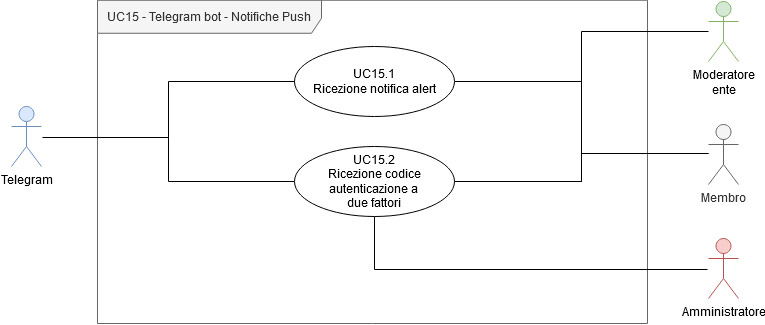
\includegraphics[scale=0.60]{res/images/uc15}
		\caption{Diagramma che descrive il processo notifica push tramite Telegram.}
	\end{figure}
		
	\begin{itemize}
		\item \textbf{Attori Primari}: Membro, Moderatore ente, Amministratore.
		\item \textbf{Attori Secondari}: \glock{Telegram}.
		\item \textbf{Descrizione}: Un utente, con l'applicazione di \glock{Telegram} attiva o in background, riceve una notifica push in base a un evento nel sistema. 
		\item \textbf{Precondizione}: L'utente ha l'applicazione di \glock{Telegram} attiva o in background e ha una chat autenticata con il \glock{bot}.
		\item \textbf{Postcondizione}: L'utente riceve una notifica da parte di \glock{Telegram}.
		\item \textbf{Scenario Principale}:
		\begin{enumerate}
			\item L'utente ha l'applicazione di \glock{Telegram} attiva o in background. 
			\item L'utente riceve una notifica push come messaggio di testo nella chat autorizzata con il \glock{bot}.
		\end{enumerate}
	\end{itemize}
	
	\subsubsection{UC 15.1 - Ricezione notifica alert}

	\begin{itemize}
		\item \textbf{Attori Primari}: Membro, Moderatore ente, Amministratore.
		\item \textbf{Attori Secondari}: \glock{Telegram}.
		\item \textbf{Descrizione}: L'utente riceve una notifica sulla chat con il \glock{bot} di \glock{Telegram} relativa ad un \glock{\glock{alert}} in cui un sensore ha superato una soglia prevista.
		\item \textbf{Precondizione}: L'utente ha l'applicazione di \glock{Telegram} attiva o in background e ha una chat autenticata con il \glock{bot}.
		\item \textbf{Postcondizione}: L'utente riceve una notifica come messaggio di testo in chat con le informazioni relative all'\glock{alert}.
		\item \textbf{Scenario Principale}:
		\begin{enumerate}
			\item L'utente ha l'applicazione di \glock{Telegram} attiva o in background.
			\item L'utente riceve una notifica che riguarda un \glock{alert} nella chat con il \glock{bot}.
		\end{enumerate}
	\end{itemize}

	\subsubsection{UC 15.2 - Ricezione codice di autenticazione a due fattori}

	\begin{itemize}
		\item \textbf{Attori Primari}: Membro, Moderatore ente, Amministratore.
		\item \textbf{Attori Secondari}: \glock{Telegram}.
		\item \textbf{Descrizione}: L'utente riceve una notifica sulla chat con il \glock{bot} di \glock{Telegram} relativa al codice per l'autenticazione a due fattori, mentre sta svolgendo l'autenticazione nella \glock{web application}.
		\item \textbf{Precondizione}: L'utente ha l'applicazione di \glock{Telegram} attiva o in background e ha una chat autenticata con il \glock{bot}.
		\item \textbf{Postcondizione}: L'utente riceve una notifica come messaggio di testo in chat con le informazioni relative al codice per l'autenticazione a due fattori.
		\item \textbf{Scenario Principale}:
		\begin{enumerate}
			\item L'utente ha l'applicazione di \glock{Telegram} attiva o in background.
			\item L'utente riceve una notifica che riguarda il codice di autenticazione a due fattori da usare come credenziale per accedere alla \glock{web application}.
		\end{enumerate}
	\end{itemize}

		% =================
		% UC 16 - [NICE]

		\subsection{UC16 - Telegram - Interazioni}
		
		%\begin{figure}[t!]
		%	\centering
		%	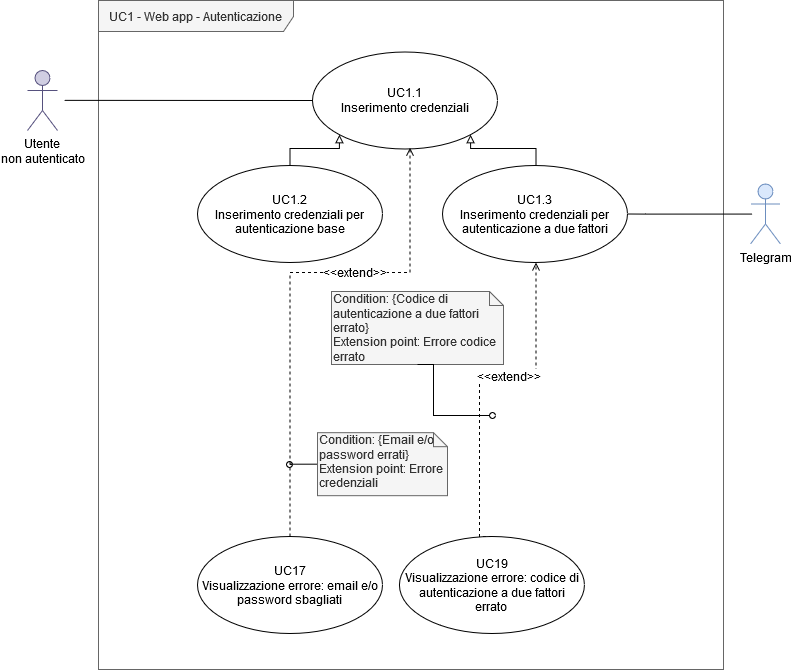
\includegraphics[height=10em]{res/images/uc1}
		%\end{figure}
		
	\begin{itemize}
		\item \textbf{Attori Primari}: Utente autenticato, Moderatore ente.
		\item \textbf{Attori Secondari}: \glock{Telegram}.
		\item \textbf{Descrizione}: Un utente mentre è nell'applicazione di \glock{Telegram} ed ha attiva la schermata di chat con il bot, può eseguire delle interazioni per gestire dispositivi remoti o ricevere informazioni particolari. 
		\item \textbf{Precondizione}: L'utente sta usando l'applicazione di \glock{Telegram} e ha una chat aperta e autenticata con il bot.
		\item \textbf{Postcondizione}: L'utente riceve un messaggio di risposta sulla chat con il bot di \glock{Telegram}.
		\item \textbf{Scenario Principale}:
		\begin{enumerate}
			\item L'utente sta usando l'applicazione di \glock{Telegram} e ha una chat aperta e autenticata con il bot. 
			\item L'utente esegue una interazione con la chat.
			\item L'utente riceve una risposta nella chat del bot.
		\end{enumerate}
	\end{itemize}
	
	\subsubsection{UC 16.1 - Invio comando e ricezione messaggio}

	\begin{itemize}
		\item \textbf{Attori Primari}: Utente autenticato, Moderatore ente.
		\item \textbf{Attori Secondari}: \glock{Telegram}.
		\item \textbf{Descrizione}: Un utente invia un comando nella chat con il bot di \glock{Telegram} e riceve una risposta in base al comando che ha inviato. 
		\item \textbf{Precondizione}: L'utente sta usando l'applicazione di \glock{Telegram} e ha una chat aperta e autenticata con il bot.
		\item \textbf{Postcondizione}: L'utente riceve un messaggio di risposta dopo aver inviato un messaggio sulla chat con il bot di \glock{Telegram}.
		\item \textbf{Scenario Principale}:
		\begin{enumerate}
			\item L'utente sta usando l'applicazione di \glock{Telegram} e ha una chat aperta e autenticata con il bot. 
			\item L'utente invia un comando tra quelli disponibili.
			\item L'utente esegue una interazione con la chat.
			\item L'utente riceve una risposta nella chat del bot.
		\end{enumerate}
		\item \textbf{Specializzazioni}:
		\begin{itemize}
			\item Invio comando /start e ricezione messaggio (UC 16.1.1)
			\item Invio comando /info e ricezione messaggio (UC 16.1.2)
			\item Invio comando /help e ricezione messaggio (UC 16.1.3)
			\item Invio comando /dispositivi e ricezione messaggio (UC 16.1.4)
			\item Invio comando di selezione di un dispositivo e ricezione messaggio con opzioni (UC 16.1.5)
			\item Invio comando di input per un dispositivo e ricezione (UC 16.1.6)
		\end{itemize}
	\end{itemize}

	\subsubsection{UC 16.1.1 - Invio comando /start e ricezione messaggio}

	\begin{itemize}
		\item \textbf{Attori Primari}: Utente autenticato, Moderatore ente.
		\item \textbf{Attori Secondari}: \glock{Telegram}.
		\item \textbf{Descrizione}: Un utente invia un comando nella chat con il bot di \glock{Telegram} e riceve una risposta in base al comando che ha inviato. 
		\item \textbf{Precondizione}: L'utente sta usando l'applicazione di \glock{Telegram} e ha una chat aperta e autenticata con il bot.
		\item \textbf{Postcondizione}: L'utente riceve un messaggio di risposta dopo aver inviato un messaggio sulla chat con il bot di \glock{Telegram}.
		\item \textbf{Scenario Principale}:
		\begin{enumerate}
			\item L'utente sta usando l'applicazione di \glock{Telegram} e ha una chat aperta e autenticata con il bot. 
			\item L'utente invia un comando tra quelli disponibili.
			\item L'utente esegue una interazione con la chat.
			\item L'utente riceve una risposta nella chat del bot.
		\end{enumerate}
	\end{itemize} 

		% =================
		% UC 17 errore auth - [NICE] 

		\subsection{UC 17 - Visualizzazione errore: email e/o password sbagliati}
		\begin{itemize}
			\item \textbf{Attori Primari}: Utente non autenticato.
			\item \textbf{Descrizione}: Dopo aver tentato di eseguire l'autenticazione nella web app, viene visualizzato un errore che segnala email e/o password errati.
			\item \textbf{Precondizione}: L'utente non è autenticato nella web app e sta tentando di autenticarsi.
			\item \textbf{Postcondizione}: L'utente rimane non autenticato.
			\item \textbf{Scenario Principale}:
			\begin{enumerate}
				\item L'utente ha inserito le credenziali richieste;
				\item Il sistema verifica le credenziali richieste;
				\item Viene visualizzato un errore che segnala email e/o password errati.
			\end{enumerate}
		\end{itemize}

		% =================
		% UC 18 errore auth - [NICE] 

		\subsubsection{UC 18 - Visualizzazione errore: account non autorizzato}
		\begin{itemize}
			\item \textbf{Attori Primari}: Utente non autenticato.
			\item \textbf{Descrizione}: Dopo aver tentato di eseguire l'autenticazione nella web app, viene visualizzato un errore che segnala che l'account con cui si sta tentando di accedere risulta essere disattivato, pertanto l'utente non è autorizzato ad accedere alla web app.
			\item \textbf{Precondizione}: L'utente non è autenticato nella web app e sta tentando di autenticarsi.
			\item \textbf{Postcondizione}: L'utente rimane non autenticato.
			\item \textbf{Scenario Principale}:
			\begin{enumerate}
				\item L'utente ha inserito le credenziali richieste;
				\item Il sistema verifica le credenziali richieste;
				\item Viene visualizzato il messaggio di errore che segnala l'errore di account non autorizzato;
			\end{enumerate}
		\end{itemize}

		% =================
		% UC 19 errore auth - [NICE]

		\subsubsection{UC 19 - Visualizzazione errore: codice di autenticazione a due fattori errato}
		\begin{itemize}
			\item \textbf{Attori Primari}: Utente non autenticato.
			\item \textbf{Descrizione}: Dopo aver tentato di eseguire l'autenticazione, viene visualizzato un errore che segnala che il codice di autenticazione a due fattori inserito è errato.
			\item \textbf{Precondizione}: L'utente non è autenticato nella web app e sta tentando di autenticarsi.
			\item \textbf{Postcondizione}: L'utente rimane non autenticato.
			\item \textbf{Scenario Principale}:
			\begin{enumerate}
				\item L'utente ha inserito le credenziali richieste;
				\item Il sistema verifica le credenziali richieste;
				\item Viene visualizzato il messaggio di errore che segnala codice errato;
			\end{enumerate}
		\end{itemize}


		% =================
		% UC 20 errore - [NICE]

		\subsubsection{UC 20 - Nessuna risposta dopo una interazione con Telegram}
		\begin{itemize}
			\item \textbf{Attori Primari}: Utente autenticato, Utente non autenticato.
			\item \textbf{Attori Secondari}: Telegram.
			\item \textbf{Descrizione}: L'utente, dopo aver eseguito una interazione con il bot \glock{Telegram}, non visualizza nessuna risposta di ritorno che si attendeva.
			\item \textbf{Precondizione}: L'utente ha eseguito una interazione con \glock{Telegram}.
			\item \textbf{Postcondizione}: L'utente non riesce a portare a termine la sua interazione e non visualizza alcun risultato.
			\item \textbf{Scenario Principale}:
			\begin{enumerate}
				\item L'utente ha tentato di eseguire una interazione su \glock{Telegram};
				\item L'utente non visualizza nessuna risposta di ritorno.
			\end{enumerate}
		\end{itemize}


		% =================
		% UC 21 errore - [NICE]

		\subsubsection{UC 21 - Visualizzazione errore: email non valida}
		\begin{itemize}
			\item \textbf{Attori Primari}: Utente autenticato.
			\item \textbf{Descrizione}: L'utente ha compilato un campo per l'email, ma l'email è già censita nel sistema, oppure è in un formato non corretto.
			\item \textbf{Precondizione}: L'utente ha compilato il campo per l'email.
			\item \textbf{Postcondizione}: L'utente visualizza un messaggio di errore specifico e non porta a termine l'azione.
			\item \textbf{Scenario Principale}:
			\begin{enumerate}
				\item L'utente ha inserito il campo per la email;
				\item Il sistema elabora la richiesta;
				\item Viene visualizzato un errore che segnala che l'email non è valida.
			\end{enumerate}
		\end{itemize}

		% =================
		% UC 22 errore - [NICE]

		\subsubsection{UC 22 - Visualizzazione errore: username Telegram non valido}
		\begin{itemize}
			\item \textbf{Attori Primari}: Utente autenticato.
			\item \textbf{Descrizione}: L'utente ha compilato un campo per l'username di \glock{Telegram}, ma lo username inserito o è già censito nel sistema, oppure è in un formato non corretto.
			\item \textbf{Precondizione}: L'utente ha compilato il campo per lo username di \glock{Telegram}.
			\item \textbf{Postcondizione}: L'utente visualizza un messaggio di errore specifico e non porta a termine l'azione.
			\item \textbf{Scenario Principale}:
			\begin{enumerate}
				\item L'utente ha inserito il campo per lo username \glock{Telegram};
				\item Il sistema elabora la richiesta;
				\item Viene visualizzato un errore che segnala che lo username \glock{Telegram} non è valido.
			\end{enumerate}
		\end{itemize}


		% =================
		% UC 23 errore - [NICE]

		\subsubsection{UC 23 - Visualizzazione errore: formato nome o cognome non valido}
		\begin{itemize}
			\item \textbf{Attori Primari}: Utente autenticato.
			\item \textbf{Descrizione}: L'utente ha compilato i campi per il nome o per il cognome, ma il formato di uno di questi due non è valido.
			\item \textbf{Precondizione}: L'utente ha compilato il campo per il nome e per il cognome.
			\item \textbf{Postcondizione}: L'utente visualizza un messaggio di errore specifico e non porta a termine l'azione.
			\item \textbf{Scenario Principale}:
			\begin{enumerate}
				\item L'utente ha inserito il campo il nome e per il cognome;
				\item Il sistema elabora la richiesta;
				\item Viene visualizzato un errore che segnala che il formato di nome o cognome non sono validi.
			\end{enumerate}
		\end{itemize}